%% 
%% ACS project dissertation template. 
%% 
%% Currently designed for printing two-sided, but if you prefer to 
%% print single-sided just remove ",twoside,openright" from the 
%% \documentclass[] line below. 
%%
%%
%%   SMH, May 2010. 


\documentclass[a4paper,12pt,twoside,openright]{report}
%TC:group tabular 1 1

%%
%% EDIT THE BELOW TO CUSTOMIZE
%%

\def\authorname{Yunjae Lee\xspace}
\def\authorcollege{St John's College\xspace}
\def\authoremail{yl457@cam.ac.uk}
\def\dissertationtitle{Measuring Brand Perception on Twitter using Context-Dependent Skip-grams}
\def\wordcount{11,513}

\UseRawInputEncoding


\usepackage{epsfig,graphicx,parskip,setspace,tabularx,xspace,verbatim,amssymb,algorithm,url,graphicx,caption,subcaption,amsmath,listings,color,enumitem,afterpage,amsfonts,cleveref,array,multirow,rotating} 

%% DECLARE COMMANDS HERE
\newcommand{\refs}[1]{}
\newcommand{\tb}{\vspace{10pt} \textbf}
\newcommand{\ti}{\textit}
\newcommand{\tx}{\texttt}
\newcommand{\nl}{\\ \\}
\newcommand{\specialcell}[2][c]{%
\begin{tabular}[#1]{@{}c@{}}#2\end{tabular}}
\DeclareFixedFont{\ttb}{T1}{txtt}{bx}{n}{10} % for bold
\DeclareFixedFont{\ttm}{T1}{txtt}{m}{n}{10}  % for normal
\definecolor{deepblue}{rgb}{0,0,0.5}
\definecolor{deepred}{rgb}{0.6,0,0}
\definecolor{deepgreen}{rgb}{0,0.5,0}
\lstset{
language=Python,
basicstyle=\singlespacing\ttm,
captionpos=b,
otherkeywords={self},             % Add keywords here
keywordstyle=\ttb\color{deepblue},
emph={MyClass,__init__},          % Custom highlighting
emphstyle=\ttb\color{deepred},    % Custom highlighting style
stringstyle=\color{deepgreen},
frame=tb,                         % Any extra options here
tabsize=1,                       % sets default tabsize to 2 spaces
stepnumber=1,                       % sets default tabsize to 2 spaces
showstringspaces=false            % 
}
\DeclareMathOperator{\sech}{sech}
\DeclareMathOperator{\csch}{csch}
\DeclareMathOperator{\arcsec}{arcsec}
\DeclareMathOperator{\arccot}{arcCot}
\DeclareMathOperator{\arccsc}{arcCsc}
\DeclareMathOperator{\arccosh}{arcCosh}
\DeclareMathOperator{\arcsinh}{arcsinh}
\DeclareMathOperator{\arctanh}{arctanh}
\DeclareMathOperator{\arcsech}{arcsech}
\DeclareMathOperator{\arccsch}{arcCsch}
\DeclareMathOperator{\arccoth}{arcCoth} 

\setcounter{secnumdepth}{5}
\setcounter{tocdepth}{5}

\begin{document}

%% FRONTMATTER (TITLE PAGE, DECLARATION, ABSTRACT, ETC) 
\pagestyle{empty}
\singlespacing
% title page information
\begin{titlepage} 

\begin{center}
\noindent
\huge
\dissertationtitle \\
\vspace*{\stretch{1}}
\end{center}

\begin{center}
\noindent
\huge
\authorname \\
\Large
\authorcollege      \\[24pt]

\includegraphics{CUni3.eps}
\end{center}

\vspace{24pt} 

\begin{center}
\noindent
\large
{\it A dissertation submitted to the University of Cambridge \\ 
in partial fulfilment of the requirements for the degree of \\ 
Master of Philosophy in Advanced Computer Science} 
\vspace*{\stretch{1}}
\end{center}

\begin{center}
\noindent
University of Cambridge \\
Computer Laboratory     \\
William Gates Building  \\
15 JJ Thomson Avenue    \\
Cambridge CB3 0FD       \\
{\sc United Kingdom}    \\
\end{center}

\begin{center}
\noindent
Email: \authoremail \\
\end{center}

\begin{center}
\noindent
\today
\end{center}

\end{titlepage} 

\newpage
\vspace*{\fill}

\onehalfspacing
\newpage
{\Huge \bf Declaration}

\vspace{24pt} 

I David Yenicelik of ETH Zürich, being a candidate for the M.Sc. ETH in
Computer Science, hereby declare that this report and the
work described in it are my own work, unaided except as may be
specified below, and that the report does not contain material that
has already been used to any substantial extent for a comparable
purpose.

\vspace{24pt}
Total word count: \wordcount

\vspace{60pt}
\textbf{Signed}: 

\vfill

This dissertation is copyright \copyright 2020 David Yenicelik. 
\\
All trademarks used in this dissertation are hereby acknowledged.



\newpage
\vspace*{\fill}

\singlespacing
\newpage
{\Huge \bf Abstract}
\vspace{24pt} 

One of the goals of Natural Language Understanding \textit{NLU} is to formalize written text in a way, such that linguistic features can be captured through computational models, which can then again be used for downstream machine learning tasks.
The most popular methodology in NLU is the use of vectors that represent written text, including word-vectors, sentence-vectors, etc. 
These vectors are often referred to as \textit{embedding} vectors, as they embed more complex concepts into a vector representation.

Because embeddings - due to their strong usage in downstream tasks - can be considered as the fundamental unit of machine learning in the domain of natural language, any shortcomings will influence the performance of the target task.
Given that language models such as BERT only capture a black-box function $f$ between input and output, our aim is to understand how the subspace organization relates to linguistic features.
We focus our analysis on \textit{semantics}, which captures a meaning within language, as this is one of the most important features of language. 
We analyse the BERT language model, as it provides a good balance between popularity, close to state-of-the-art performance, and generalizability to other modern language models.
\\

Our main contributions are the following: (1) We test for linear separability and ability to partition the space into semantic clusters within the sampled BERT vectors.
We show that while linear separability is possible, it is nearly impossible to find modes in the data which correspond to semantic classes that are as cleanly as defined by WordNet.
We conclude that BERT organized the embedding vectors imminently by context, and very little by semantics alone.
This can easily introduce undesirable properties such as strong sentiment, leading to considerable bias in downstream tasks.
(2) We analyze the relationship between part-of-speech and semantics. 
We show that these show a strong correlation in languages and that modern language models capture this strong correlation.
This affects the conclusion of some related work which had analysed language models which capture semantics, but which did not account for the correlation between part-of-speech and semantics.
(3) Finally, we introduce additional parameters for words whose sampled embedding vectors have high variance over the embedding space.
We investigate what downstream tasks are most affected  and use this as a proxy to understand what information is captured the most by the directions with high variance. \\

\newpage
\vspace*{\fill}


\pagenumbering{roman}
\setcounter{page}{0}
\pagestyle{plain}

\singlespacing
\tableofcontents
\listoffigures
\listoftables

%\onehalfspacing
\setstretch{1.4}

%% INTRODUCTION

\chapter{Introduction}
\pagenumbering{arabic} 
\setcounter{page}{1} 

Brand is a collection of experiences regarding the product, employees and services offered by a company. Competing companies in the same product category often offer goods with a similar price range and functionalities. As a result, brand can be a key differentiating component in consumers' choice of one product over another~\cite{makens65}. Blind taste tests often reveal how customers fail to tell the brands apart from the products alone. A recent study shows that when given three tastings of unlabelled beer, two of which from the same brand, most people could not reliably single out the third tasting~\cite{almenberg14}. The degree to which brand affects purchase decisions is also demonstrated by another study with wine, where wine drinkers are shown to be willing to pay more for a label that is difficult to pronounce~\cite{mantonakis13}.
\nl
Marketing professionals employ various methodologies to discover how their brand is perceived. These include personal interviews and focus groups, where a group of people are asked to discuss their opinions of a certain company and its services. However, such qualitative techniques are not only inefficient in gathering data but also inaccurate, bringing into question the statistical significance of the hypothesis derived as a result. 
\nl
This thesis proposes to automate this process by building a language model from an English corpus mined from Twitter. As social networks become more pervasive and personal, on platforms such as Twitter, utterances are now often paired with metadata about the speaker, \ti{e.g.} time, location, gender and even politifical preferences. With a corpus of Tweets tagged with such a rich set of information, I trained a neural network language model that is sensitive to the contexts of the speaker. The aim of this project is then to design a system capable of answering empirical questions such as ``what is the brand most associated with cars for women aged between 20 and 25 living in New York?" I will demonstrate the validity of the model by comparing its performance to that of context-insensitive models, on test data designed to measure how well models capture the inter-speaker variability of language. From the brand analytics standpoint, this method provides insights into consumer perception for specific demographics, enabling highly fine-grained, targeted marketing. Also, the language model used in this thesis enables \ti{online learning}; in other words, incoming training data can be fed into the model to continue training and update its parameters. Hence, it is also possible to examine the temporal change in brand semantics over time.
\nl
I used a neural network language model known as the \ti{Skip-gram model}, augmented with context information. I give a brief overview of vector space models and neural language models in Chapter \ref{ch2}, as well as a high-level overview of the Skip-gram model architecture. User-composed contents in online microblogs contain a huge degree of noise; hence compiling a sizeable and meaningful dataset is a challenge. Chapter~\ref{ch3} explains the procedure of mining a corpus from Twitter and preprocessing the data to obtain high quality corpora. I will describe the model architecture and the training process in Chapter~\ref{ch4}, where I also detail various optimisation techniques used to either reduce the space requirements and speed up the training process. Finally, I confirm the capability of the model to represent linguistic variation amongst different demographics via a quantative evaluation with several carefully designed test sets. I finish the dissertation with some interesting qualitative results and perception rankings of brands in the US across 18 product categories computed by the model. 
\nl
The main contributions of this work are:
\begin{itemize}
	\item Extending the state-of-the-art language model to accommodate different categories of user contexts.
	\item Suggesting an efficient and accurate technique in computational brand analytics that represents online user sentiment well. 
	\item Showing that it is possible extract a huge corpus from Twitter whose content are meaningful enough to construct a language model.
\end{itemize}

\chapter{Background}
\label{ch2}

This chapter gives a brief overview of the background of this work. Earlier work on Computational Brand Analytics (CBA) using machine learning techniques is described in \S\ref{ch2s1}. This is followed by a survey of recent work on social applications of Natural Language Processing (NLP). After a few pointers into papers used in text normalisation, I move on to briefly outline several approaches to language modelling, finishing the chapter with a description of specific model implementation adopted as a starting point of this project.

\section{Brand analytics and social NLP}
\label{ch2s1}

Early work on Computational Brand Analytics dates back to Kuehn's work~\cite{kuehn76}, in which he described brand shifting as a stochastic learning process based on consumers' past purchase patterns. Gupta (1988) took this hypothesis further and modelled the effect of sales promotion in detail, with the impact of market indices expressed as an exponential interpurchase time model, a multinomial logit model for brand selection and cumulative logit model for quantity of purchase~\cite{gupta88}.
\nl
More recent work in marketing research applied Bayesian Inference to predict product sales dynamics from Facebook applications data before launching, with the hypothesis that true consumer network characterstics can be inferred from aggregated diffusion patterns observed in the market~\cite{trusov13}. Tirunillai \ti{et. al} (2014) applied Latent Dirichlet Allocation (LDA) to manually collected 350,000 customer reviews in five market categories (personal computers, cellular phones, footwear, toys and data storage)~\cite{tirunillai14, tirunillai12}. They showed that market sentiment can be inferred from user generated contents (\ti{e.g.} social networks, product reviews and bulletin boards) by extracting a few key latent dimensions within consumer satisfaction space about the quality of products.
\nl
As more of life is presented online and recorded in natural language,  there has been active research in the NLP literature to make interesting inferences in social science. Thomas \ti{et al.} (2006) used Support Vector Machines (SVM) and Graph Mincuts to determine whether Congress suports or opposes the proposed legislation from the debate transcript~\cite{thomas06}. Another recent work attempts to predict the success of a book based on statistical analysis of its literary style with SVM~\cite{ashok13}. 
\nl
However, to my knowledge, there has been no published work that applies of ML and NLP techniques to modelling brand perception of specific demographics. The goal of this thesis is a brand analytics model that produces informative and insightful results from a marketing perspective.

\section{Vector space and language model}

\tb{Vector space model}

Distributional semantics is a branch of linguistic semantics that is based on the distributional hypothesis: `words that often appear with similar contexts have similar meaning'~\cite{harris54}. Here contexts mean words that appear close to the target word (usually within a few words). Distributional semantic analysis is often implemented concretely with a Vector Space Model (VSM), where a word is represented by a vector residing in a high dimensional space. 
\nl
Each dimension of the vector space could either be mapped to an actual word (the magnitude of a vector on the dimension then denotes the relative frequency with which a target word co-occurs with this particular context word), or some abstract meaning that does not correspond to an actual word but could potentially be expressed with multiple different words. Both Latent Semantic Analysis (LSA) and neural network word embeddings involve dimensions in vector space that do not correspond to concrete words. 
\nl
Vector space models have an appealing property that similarity between two words can easily derived from the corresponding vectors. The most common choice is cosine similarity, which for vectors $\mathbf{a}$ and $\mathbf{b}$:
$$ {sim}(\mathbf{a},\mathbf{b}) = \frac{\mathbf{a}\cdot\mathbf{b}}{\|\mathbf{a}\| \cdot \|\mathbf{b}\|} = \cos(\theta),$$
where $\theta$ is the angle between the two vectors. The similarity value ranges from $-1$ to $1$ and is greater if two words are more similar in meaning. For example, we would expect $sim(dog,cat)>sim(dog,democracy)$ for any reasonable model.

\tb{N-gram language model}

In statistical language processing, n-gram models have been the state of the art for language modelling until recent years. On the most basic level, training an n-gram model amounts to counting the relative frequencies of word sequences of length $n$ appearing in a document. The model then predicts the probability of a new document $w_1^T$ as
\begin{equation}
\hat{P}(w_1^T)=\prod_{t=1}^T{\hat{P}(w_t|w_{t-n+1}^{t-1})}
\label{ch1:nnlm}
\end{equation}
\noindent where $w_i$ is the $i^{th}$ word in the document, $T$ is the length of the document and $w_i^j = (w_i, w_{i+1}, ..., w_j)$. $\hat{P}$ denotes estimated probability. This Markov model serves as an approximation of a true language model, but gives surprisingly good results. Concretely, back-off techniques are often used for good performance in order to combat data sparsity.
\nl
There are two obvious drawbacks to the n-gram model. Firstly, the n-gram model is an approximation to the true language model therefore is inevitably limited, as natural language writings are often coherent and humans take advantage of not only the previous word but also the previous sentence and the previous paragraph to understand the next word. Also, n-gram models are unable to take word similarity into context when making predictions: having seen \ti{I have to walk my dog at the park} in the training corpus before, we expect the model to predict \ti{I have to walk my cat in the garden} with reasonably high probability. This, however, is not achieved by n-gram models if the number of co-occurrences for one bigram is smaller than the other. The neural language model, explained in the next section, overcomes this by internally constructing a mapping from words to a vector representation, then performing prediction using the representations. As a result, different words with similar meanings get mapped to close vector representations first.

\tb{Neural language model}

Recent years have seen an active increase of applications of neural networks in language modelling, since the pioneering work by Bengio, Ducharme, Vincent and Jauvin~\cite{bengio03}. Similarly to n-gram models, Bengio's neural language model represents the conditional probability of the next word given the previous sequence of words. 

\begin{figure}[htbp]
    \centering
    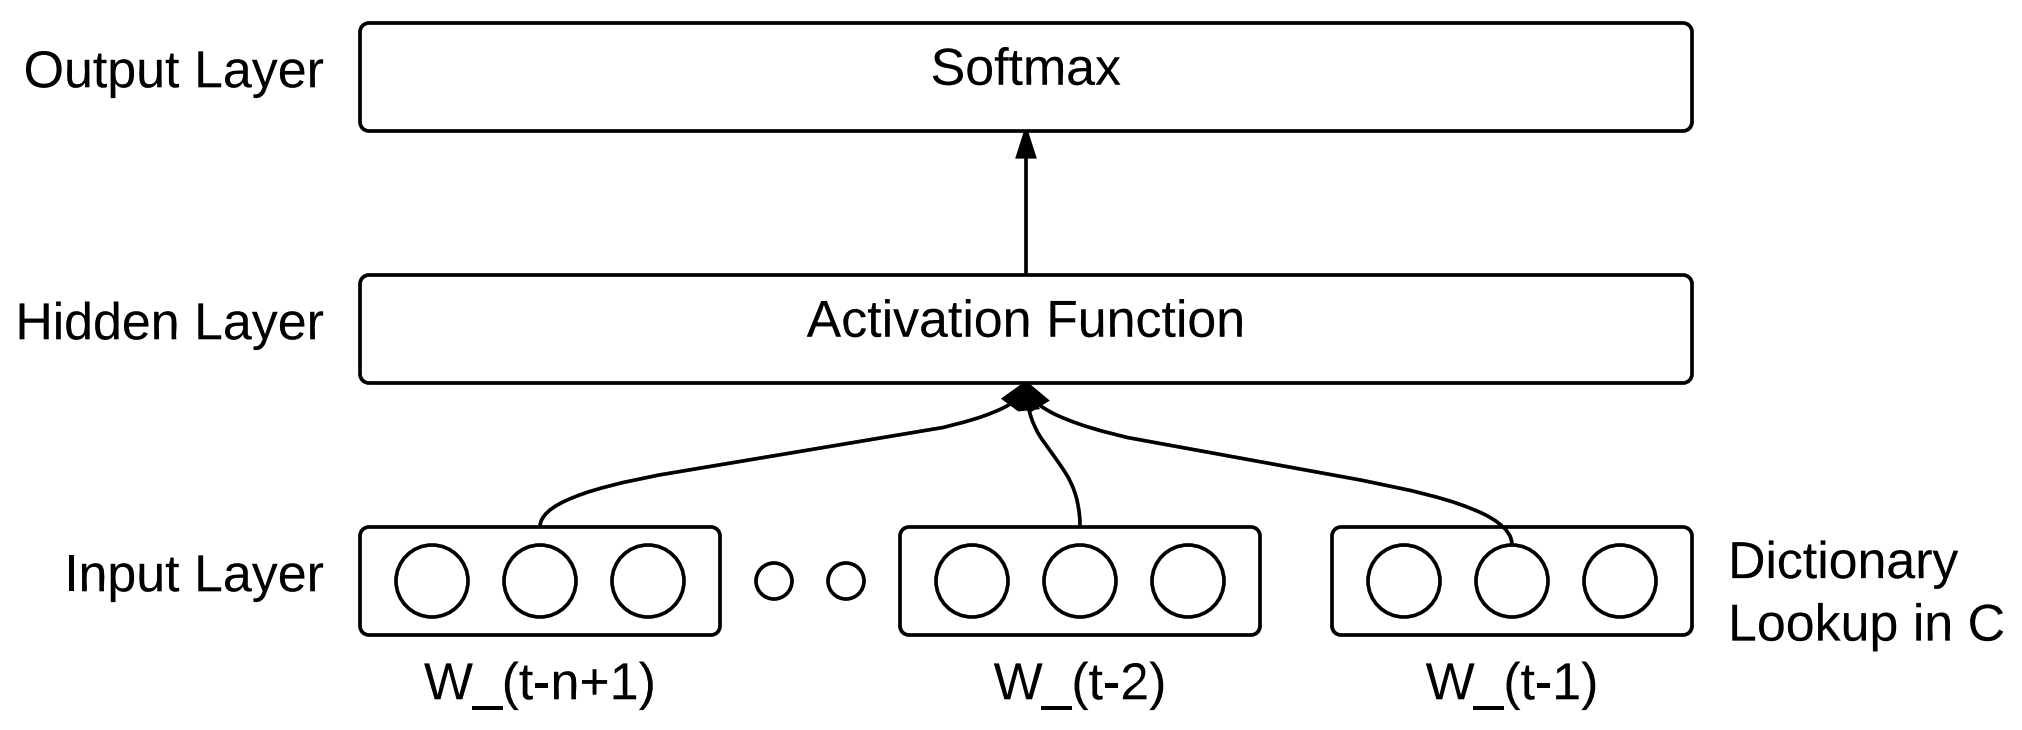
\includegraphics[width=12cm]{figs/nnlm2.png}
    \caption[Neural network architecture.]{Neural network architecture. At the input layer are one-hot vectors that index into particular words in the embedding matrix $C$. The word embeddings are concatenated and passed to the activation function.}
    \label{fig:chap2:nnlm}
\end{figure}

A neural language model has two parts: an encoder and a predictor (see Figure~\ref{fig:chap2:nnlm}). An encoder, often called \ti{autoencoder} in the neural network literature, is an unsupervised feedforward network that learns sparse representations of words. A trained autoencoder produces a mapping $C$ from a word $w_t \in V$ to a vector representation, such that $C(w_t) \in \mathbb{R}^m$. This serves as a dimensionality reduction technique as the learned word representation (called \ti{word embeddings}) is often low-dimensional hence compact. Using the word embeddings learned by the autoencoder, the predictor learns the function $f$ that predicts the next word, given the embeddings of previous $n-1$ words:
$$\hat{P}(w_1^T)=\prod_{t=1}^T{f(C(w_t),C(w_{t-1}),\cdots,C(w_{t-n+1}))},$$
\noindent where $f(w_t, \dots, w_{t-n+1}) = \hat{P}(w_t|w_{t-n+1}^{t-1})$ and $\sum_{i=1}^{|V|}{f(i,w_{t-1},\dots,w_{t-n+1}) = 1.}$

Stochastic gradient ascent and backpropagation algorithm is often used for training, with a goal to maximise the regularised log likelihood of the training corpus, \ti{i.e.}
$$L=\frac{1}{T}\sum_t^{}{f(w_t,w_{t-1},\ldots,w_{t-n+1};\theta)+R(\theta)},$$ where
\noindent $\theta$ is the parameter set including the embedding matrix $C$ and some additional parameters related to the predictor function~\cite{rumelhart88}. The regularisation term is denoted as $R(\theta).$ At the output layer, the neural network computes the softmax function of the incoming activation to ensure that all probabilities sum to one.
\begin{equation}
\hat{P}(w_t|w_{t-1},\dots,w_{t-n+1}) = \frac{e^{y_{w_t}}}{\sum_i^{|V|}{e^{y_i}}},
\label{eq:ch2:output_layer}
\end{equation}
\noindent where $y_i$ for each word $i$ is computed as $y=Ax+\tanh(b+Cx)$ with parameters $A, b$ and $C$.
\nl
Stochastic gradient ascent on the neural network is performed to learn the parameters $\theta$, with an update rule:
\begin{equation}
\theta \leftarrow \theta + \eta\frac{\partial\log\hat{P}(w_t|w_{t-1},\dots,w_{t-n+1})}{\partial\theta},
\label{eq:ch2:sgd}
\end{equation}
where $\eta$ is the learning rate. Gradient ascent approaches local maxima by taking small steps towards the direction where the ascent is steepest. Note that update to the parameter is made after each training example, approximating the true gradient with the gradient of a single example. This implies that only a small fraction of the parameters need to be updated after each example.

\tb{Skip-gram language model}

Recently, Mikolov \ti{et al.} developed a novel neural network model called the skip-gram model~\cite{mikolov13}. Their approach uses every word to predict its every neighbour word (the standard neural language model in contrast only uses previous words to predict the current word), where a neighbour word is a word appearing within a predefined distance to the context word. This structure hence allows \ti{skips} between the neighbour word and the context word. Therefore, the skip-gram model moves away from the n-gram paradigm by allowing prediction of a word with a word that occurs later. 
\nl
This model gives state of the art performance in word similarity tasks while requiring lower computational cost compared to other neural architectures. The authors also demonstrate the ability of the model to capture interesting relationships with learnt word embeddings, \ti{e.g. vec(`King') $-$ vec(`Man') $+$ vec(`Woman')} is closest to \ti{vec(`Queen').}

\begin{figure}[htbp]
    \centering
    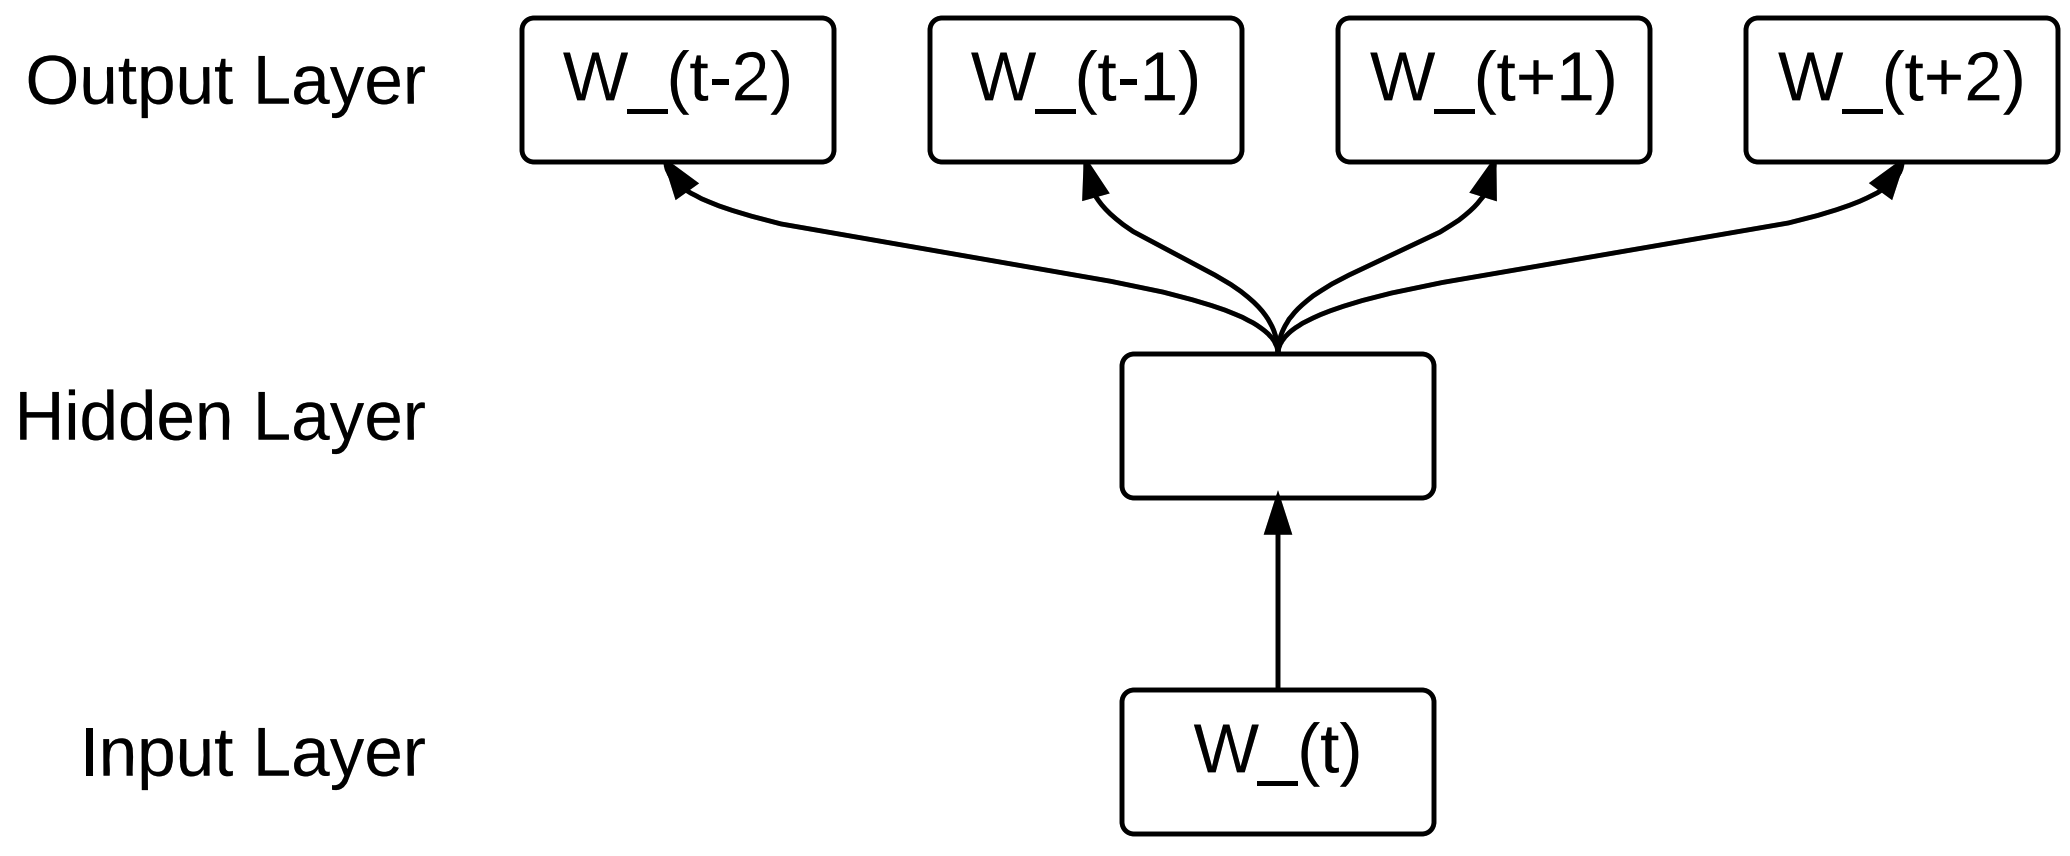
\includegraphics[width=10cm]{figs/skipgram2.png}
    \caption[Skip-gram network architecture.]{Skip-gram network architecture. Every word is used to predict the identities of its every neighbour word in both directions (not just the words after it).}
    \label{fig:chap2:skipgram}
\end{figure}

\tb{Recent advances}

While the skip-gram remains the state-of-the-art for word embeddings, it has also been shown that learning embeddings of paragraphs gives superior performance in text classification and sentiment analysis tasks compared to the bag-of-words approach~\cite{le14}. On the other hand, Vilnis \ti{et al.} demonstrated the advantages of moving away from learning representations of words as points in vector space, and instead suggested learning a Gaussian distribution over word embeddings to better handle uncertainty of word meanings. They show that representing entailment between concepts as KL divergence between two distributions gives good performance in entailment prediction tasks~\cite{vilnis14}.

\section{Resources}

Mikolov \ti{et al.} released an implementation of the skip-gram model in C, which takes a corpus as an input and produces a dictionary of learned word embeddings as output\footnote{\url{https://code.google.com/p/word2vec/}}. Rehurek took this implementation and ported it into Python. By optimising heavy loops in the core backpropagation module in Cython and multithreading, his implementation offers both readability and performance improvement compared to the original release in C.\footnote{\url{https://github.com/piskvorky/gensim/blob/develop/gensim/models/word2vec.py}} Cython is a C-extension for Python that allows calling C/C++ code from Python code, achieving C-level performance.\footnote{\url{http://cython.org/}}. It also interacts efficiently with large datasets in Python such as NumPy arrays. As Python provides well-integrated libraries with to interact with Twitter API and SQLite\footnote{\url{https://www.sqlite.org/}} database API, I took Rehurek's implementation of the skip-gram model as a starting point and augmented it with functionalities to support context-dependent word embedding matrices.

\chapter{Data Mining and Preprocessing} \label{ch3}

From the very outset of the project, it was clear that obtaining a huge volume of tweets tagged with meaningful context information is key to its success. I outline the work involved in obtaining such a corpus in three parts: mining the tweets, preprocessing the content of the tweets and finally predicting the metadata of users based on available user information.
\nl
Cleansing social media data with a high degree of noise constitutes a research topic of its own. As social media data is heavily used in the NLP community, increasing amount of research is conducted in text normalisation directed specifically towards microblogs . Yang and Eisenstein (2013) presented a log-linear framework with Monte Carlo training for unsupervised text normalisation~\cite{yang13}. Several simple decision list classifiers were used in this thesis to predict several types of user metadata.
\nl
I finish the chapter with a detailed breakdown of demographic statistics of the training data, namely distributions of location, age and gender of the tweets corpus.

\section{Mining the corpus}

This process involved collecting a corpus of tweets of 8.8 billion tokens from 623 million tweets gathered over a period of approximately three months (August to November 2014\footnote{This thesis started as a summer internship at the Natural Language and Information Processing Group of the Computer Laboratory during this period, with Douwe Kiela and Steven Ghoussain.}). Tweepy library\footnote{\url{https://github.com/tweepy/tweepy}} was used to access the Twitter API from Python, and collected data was compiled into an SQLite database. 
\nl
I decided to perform tweet content normalisation and user metadata prediction separately, rather than both at the same time for each tweet. As most users tweet multiple times, it saves computation to perform user metadata prediction only once. This implied maintaining two separate databases: one for tweets and another for users who composed the tweets.

\tb{Tweets database}

During initial mining from the Twitter API, I extracted seven fields for each tweet, with description provided below.

\begin{table}[htbp]
\begin{center}
\begin{tabular}{ c | c | l }
 Field & Datatype & Description \\ \hline 
 \tx{id\_str} & \tx{text} & Numeric string identifier for individual tweets. \\ 
 \tx{coordinates} & \tx{text} & Location of the tweet in coordinates. \\
 \tx{created\_at} & \tx{text} & Time of authorship.\\
 \tx{place} & \tx{text} & Location of the tweet in plain text.\\
 \tx{retweeted} & \tx{integer} & Number of retweets received.\\
 \tx{content} & \tx{text} & Content of the tweet.\\
 \tx{uid\_str} & \tx{text} & Numeric string identifier for individual users.\\   \hline
\end{tabular}
\end{center}
\caption{Tweets database fields}
\label{tab:chap3:tweets.db}
\end{table}

\noindent Once the tweets database has been compiled, I normalised \tx{content} of each tweet. I fed the normalised content into the neural network when training the model. 

\tb{Users database}

After the tweets database has been mined, I took the unique set of \tx{uid\_str} in the tweets database. Then, for each \tx{uid\_str} I extracted seven additional fields from Twitter and compiled them into a users database.

\begin{table}[htbp]
\begin{center}
\begin{tabular}{ c | c | l }
 Field & Datatype & Description \\ \hline 
 \tx{uid\_str} & \tx{text} & Numeric string identifier of the user.\\   
 \tx{name} & \tx{text} & Full name.\\   
 \tx{screen\_name} & \tx{text} & Username on Twitter.\\   
 \tx{location} & \tx{text} & Location of the user.\\   
 \tx{time\_zone} & \tx{text} & Timezone of the user's location.\\   
 \tx{lang} & \tx{text} & The language of user's choice.\\   
 \tx{followers\_count} & \tx{integer} & The number of people following the user.\\   
 \tx{description} & \tx{text} & \specialcell{A plain text description about\\the user given by himself/herself.} \\ \hline
\end{tabular}
\end{center}
\caption{Users database fields}
\label{tab:chap3:users.db}
\end{table}

\noindent Once the database such as Table~\ref{tab:chap3:users.db} has been compiled for all users in the tweets database, user metadata was predicted from the information available in the users database. Location was inferred from \tx{time\_zone} and \tx{location}, gender was deduced from \tx{name} and age estimated from the \tx{description} field (see Section~\ref{prediction} for details).

\section{Tweet normalisation}

Preprocessing a corpus of this size will not be trivial. To obtain a dataset of reasonable quality within a given timeframe, a careful balance between normalisation quality and latency was needed. A pipeline\footnote{Implemented by Steven Ghoussain during the summer internship.} of preprocessing techniques was performed to the \tx{content} of each tweet in the following order. Some key decisions regarding the precision of normalisation are discussed below.

\tb{Removing duplicate characters}

A phenomenon particularly common in tweets is duplication of certain characters to express excitement or agreement, such as \tx{loool} and \tx{sweeeeeet!}. This was addressed with a concise and efficient character-level script that reduces substrings consisting of more than two consecutive, identical characters into a single character. Hence, \tx{loool} and \tx{greaaaaat} are mapped to \tx{lol} and \tx{great} respectively. 

\tb{Expanding abbreviations and contractions}

Abbreviations and contractions are extensively used in online microblogs. To correctly expand such occurrences back to their standard forms, I constructed a list of major contractions\footnote{\url{http://grammar.about.com/od/words/a/EnglishContractions.htm}} and online acronyms\footnote{Used entries combined from \url{http://www.netlingo.com/acronyms.php} and \url{http://www.webopedia.com/quick_ref/textmessageabbreviations.asp}}. For example, \tx{brb} and \tx{y'all could've} were converted to \tx{be right back} and \tx{you all could have}.

\tb{Spelling Correction}

Another key source of noise in online microblogs is spelling mistakes. To address this, I have used an out-of-the-box solution, a Python spell-checker package known as Pyenchant\footnote{\url{http://pythonhosted.org/pyenchant/}} that also suggests likely words given an incorrect spelling of a word. For example, given \tx{helo}, some examples of suggested possible alternative words are: \tx{hello, halo} and \tx{hell}. 

\tb{Lowercasing}

Online microblog users tend to ignore casing rules and write entirely in lowercase, and this is more pronounced among personal users than corporate or group users on social media. Therefore, following a common approach in Tweet normalisation, I have opted to lowercase all tokens for simplicity and performance, at the expense of some minor loss of accuracy.

\tb{Named entity recognition}

\begin{table}[htbp]
\begin{center}
\begin{tabular}{ c | c }
 Original & Preprocessed \\ \hline
 \tx{yeeeees} & \tx{yes}  \\  
 \tx{shouldve} & \tx{should have} \\
 \tx{yolo} & \tx{you only live once} \\
 \tx{pizza hut} & \tx{pizza\_hut} \\ 
 \tx{@disneyparks} & \tx{disneyland} \\ 
  \tx{\$six} & \tx{six\_flags} \\ \hline
\end{tabular}
\end{center}
\caption{Tweet normalisation results.}
\label{tab:chap3:preprocessing_results}
\vspace{-0.1cm}
\end{table}

As this project attempts to model the semantics of brand names in a context-sensitive way, it is of prime importance to correctly recognise key named entities in tweets. Stanford's CRF NER system was initially chosen to perform the recognition task\footnote{\url{http://nlp.stanford.edu/software/CRF-NER.shtml}}. However, visual inspection of results revealed that Stanford's system is too inadequate for recognising entities in online microblogs, presumably because the system was trained on newswire transcripts and articles which are vastly different from the majority of written language found online. Another issue with Stanford's NER system was that its latency was too big to run on the entire tweets database.
\nl
Therefore, I have constructed a named entity dictionary of key interest words. These words include brand names, sports team names and additional words that are expected to bear varying semantic representation for different demographics.
\nl
A key function of Twitter is that users can personally `mention' other users by prepending the @ sign to the desired person's username. As many companies and sports teams have accounts on Twitter, this functionality is actively utilised by users to mention companies in their discourse. Another way to discuss (usually the financial aspects of) a company on Twitter is to use the \$ symbol prepended to the NASDAQ ticker symbol of the company. See the following microblogs for examples of both. 
\nl
\fbox{\begin{minipage}{\textwidth}
\tx{Custom @adidas gear showed up today! Even our big men have swag! Look good, Play good! \#BeTheStandard \#SpeedKills}. 
\end{minipage}}  

\fbox{\begin{minipage}{\textwidth}
\tx{Jeez that interview last night on @MadMoneyOnCNBC with Doug Parker from \$AAL really crushed this group}
\end{minipage}}

As both methods are major channels of communication on Twitter, these occurrences were identified and converted to original names of entities in the recognition stage. See Table~\ref{tab:chap3:preprocessing_results} for the input and output of the normalisation module.

\section{User metadata prediction}
\label{prediction}

With the user database mined as in Table~\ref{tab:chap3:users.db}, the metadata of each user was predicted from the information available in the database, to be later merged with each tweet composed by that user so that each utterance in the final database is tagged with corresponding user metadata. Users on Twitter provide personal information in a semi-organised manner, with related information often scattered across several fields (\ti{e.g.} some users describe their location in the \tx{description} field, rather than \tx{location}). 

\tb{Location}

First and foremost, a gazeteer of location names was compiled, containing: 4409 major US cities, 749 major Canadian cities, 1258 major UK cities and 71 major world cities by population, in addition to 194 countries and 64 American/Canadian states.
\nl
User location was classified by detecting location keywords in \tx{location} and \tx{time\_zone} fields. Hypothesied user location was arranged into three new fields: \tx{city, state} and \tx{country}, where the \tx{state} is only meaningful in certain countries, namely US and Canada. A high-level algorithm for predicting a user's location is given in Algorithm~\ref{alg:chap2:location_algorithm}.

\begin{table}[htbp]
\begin{center}
\begin{tabular}{ c c | c c c }
 \tx{location} & \tx{time\_zone} & \tx{city} & \tx{state} & \tx{country} \\ \hline
 & Netherlands &  & & netherlands \\
 & Bangkok & bangkok & & thailand \\
 Indiana & US \& Canada & & indiana & us \\
 Boulder & US \& Canada & boulder & colorado & us \\ 
 Houston, TX & US \& Canada & houston & texas & us \\ \hline
\end{tabular}
\end{center}
\caption[Examples of location prediction results.]{Examples of location prediction results. Three columns on the right list \ti{inferred} user properties.}
\label{tab:chap3:location_results}
\end{table}

\noindent Table \ref{tab:chap3:location_results} shows predicted locations of users from some example input fields; namely, five different types of location descriptions are captured by the prediction module.
 
\begin{enumerate}[itemsep=-9pt]
	\item US/Canada
	\begin{enumerate}[itemsep=-9pt]
		\item (\tx{city, state}): If a token is a valid state in US, the previous token is taken to be \tx{city}. Then, \tx{city, state} and \tx{country} are updated accordingly.
		\item \tx{city}: if a token is recognised as a valid city in US, then \tx{city, state} and \tx{country} are updated accordingly.
		\item \tx{state}: if a token is a valid US state, \tx{state} and \tx{country} are updated accordingly.
	\end{enumerate}
	\item World
	\begin{enumerate}[itemsep=-9pt]
		\item \tx{country}: if a token is a valid country name, \tx{country} is updated accordingly.
		\item \tx{city}: if a token is avalid city name, \tx{city} and \tx{country} are updated accordingly. 
	\end{enumerate}
\end{enumerate}

\begin{algorithm}[htbp]
\begin{enumerate}
	\item Search for country names in \tx{location} and \tx{time\_zone}.
	\item If country is either US, Canada or not found, search for US/Canadian state names.
	\item If state is found, the word preceding the state is assumed to be city.
	\item If a country but no state is found, search for world city names (non US/Canada).
\end{enumerate}
\caption{Outline of location prediction algorithm.}
\label{alg:chap2:location_algorithm}
\end{algorithm}

\tb{Gender}

Gender classification was performed based on users' first names in the \tx{name} field. A simple decision list classifier was constructed using the US census data regarding popularities of male and female first names\footnote{\url{http://www.census.gov/topics/population/genealogy/data/1990_census/1990_census_namefiles.html}}. The data gives frequency in percent of a given first name for a given gender, \ti{e.g.} `James' consisted of approximately 3.32\% of all American males at the time of the survey. For gender-ambiguous first names such as Charlie, two genders were compared based on the relative frequency and the gender with the higher relative frequency was taken. See Table~\ref{tab:chap3:gender_results} for some examples for gender prediction.

\begin{table}[htbp]
\vspace{-0.5cm}
\begin{center}
\begin{tabular}{ c | c }
 \tx{name} & \tx{gender} \\ \hline
 Cristian Rivas & male \\
 Quinton Cameron & male \\
 Robbie Macgregor & female \\
 jen & female \\ 
 adriana & female \\ \hline
\end{tabular}
\end{center}
\caption[Examples of gender prediction results.]{Examples of gender prediction results. The \tx{gender} field was predicted from the \tx{name} field.}
\label{tab:chap3:gender_results}
\vspace{-0.3cm}
\end{table}

Approximately 6\% of the corpus was tagged with hypothesised gender information (see Figure~\ref{fig:chap3:gender}).

\tb{Age}\footnote{Implemented by Steven Ghoussain during the summer internship.}

Twitter does not ask for users' date of birth or age during signup. Hence, this information tends to be included in the \tx{description} field, often at the beginning rather than at the end. The age predictor was designed to detect possible occurences of age in the first four characters in the \tx{description} field. 

\begin{table}[htbp]
\begin{center}
\begin{tabular}{ c | c }
 \tx{description} & \tx{age} \\ \hline
 18, \#SandrasSoldiersForever & 18 \\
 I'm 16 \#TeamMindless.MUSIC IS LIFE. & 16 \\
 3rd Year CTP student. Chairman of @MMUCBasiks. &  \\
 10 days till I meet my idols & \\ \hline
\end{tabular}
\end{center}
\caption[Examples of age prediction results.]{Examples of age prediction results. \tx{age} column shows hypothesised age of the user.}
\label{tab:chap3:age_results}
\end{table}

\noindent Note that a basic sanity check was performed so that numbers that can clearly not be an age were eliminiated, including ordinal numbers and quantities (\ti{e.g.} {12 months}). Approximately 0.25\% of the tweets database (22 million tweets) were tagged with age metadata.

\section{Tweet demographic statistics}

\afterpage{
\begin{figure}
	\vspace{-13mm}
	\hspace{-10mm}
        \begin{subfigure}[b]{8cm}
                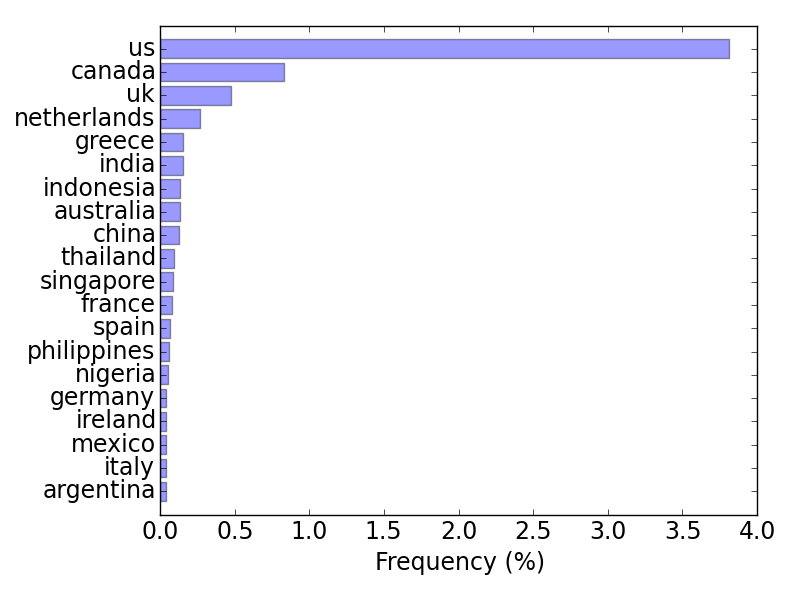
\includegraphics[width=8cm]{figs/chap2/country.png}
		\captionsetup{justification=centering}
                \caption{Top 20 countries with the largest number \\ of tweets.}
                \label{fig:chap3:countries}
        \end{subfigure}%
        ~ %add desired spacing between images, e. g. ~, \quad, \qquad, \hfill etc.
          %(or a blank line to force the subfigure onto a new line)
        \begin{subfigure}[b]{8cm}
                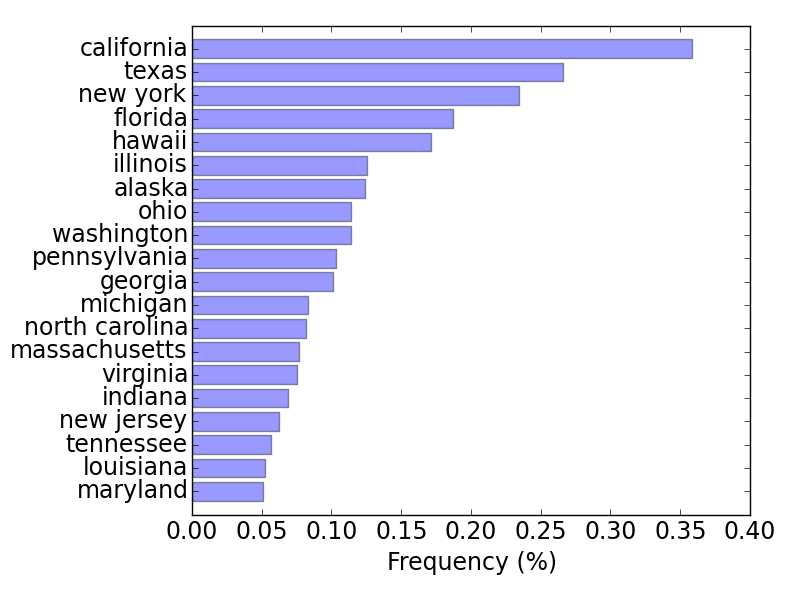
\includegraphics[width=8cm]{figs/chap2/state.png}
                \captionsetup{justification=centering}
                \caption{Top 20 states with the largest number \\of tweets within US/Canada.}
                \label{fig:chap3:states}
        \end{subfigure}
	\captionsetup{justification=centering}
        \caption{Distribution of countries and US/Canadian states.}
        \label{fig:chap3:location_dist}
%\end{figure}
%\begin{figure}
	\hspace{-10mm}
        \begin{subfigure}[b]{8cm}
                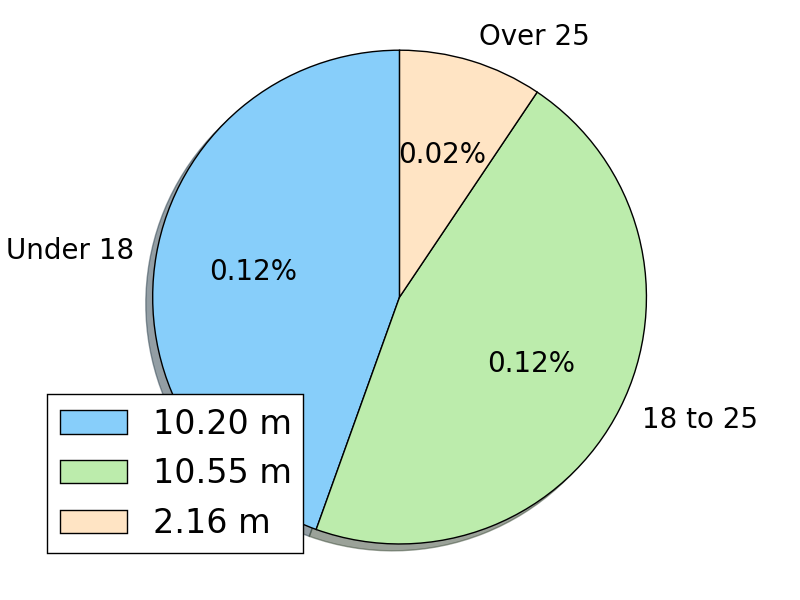
\includegraphics[width=8cm]{figs/chap2/age.png}
                \caption{Age distribution of tweets}
                \label{fig:chap3:age}
        \end{subfigure}%
        ~ %add desired spacing between images, e. g. ~, \quad, \qquad, \hfill etc.
          %(or a blank line to force the subfigure onto a new line)
        \begin{subfigure}[b]{8cm}
                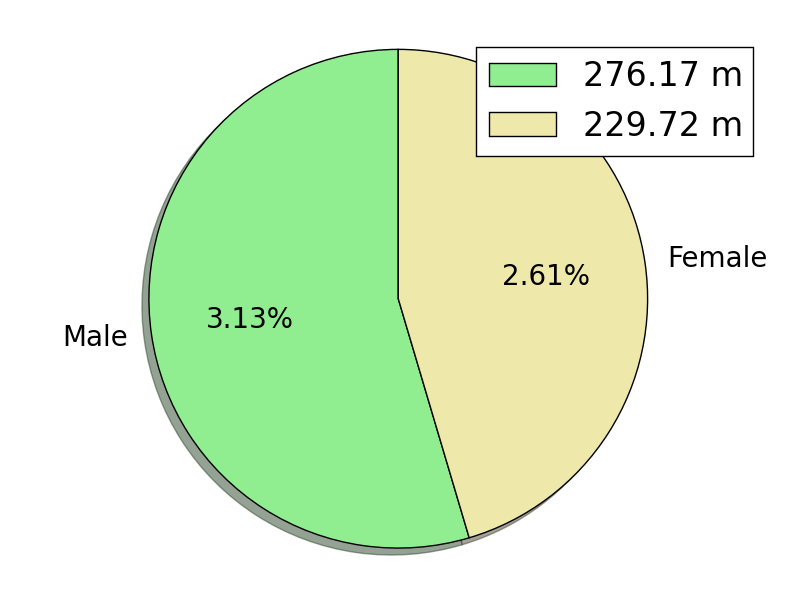
\includegraphics[width=8cm]{figs/chap2/gender.png}
                \caption{Gender distribution of tweets.}
                \label{fig:chap3:gender}
        \end{subfigure}
	\captionsetup{justification=centering}
        \caption[Distribution of age and gender.]{Distribution of age and gender.\footnotemark}
        \label{fig:chap3:age_gender_dist}
\end{figure}
\footnotetext{Pie patches show proportions with respect to entire tweets. Numbers in legends denote the number of tweets with corresponding context.}        
}
Once every tweet has been normalised and every user's metadata predicted, each tweet in the tweets database was tagged with corresponding user's metadata (if available). Among 623 million tweets that have been compiled, the frequency of those with context information was determined and plotted on a chart. Figure~\ref{fig:chap3:countries} gives the histogram for the distribution of countries among tweets geotagged with country. Unsurprisingly, the US has the largest number of tweets, followed by Canada, UK and Netherlands. Within US and Canada, California constitutes the largest state in terms of the number of tweets, with Texas, New York and Florida next in rank. The top five results for states aligns with the order of US states by population. 

In terms of age distribution, the young demographic did comprise the majority of the online population, with people under 25 making up more than 90\% of people with predicted age. Gender distribution shows that tweets composed by males slightly outnumber tweets by their female counterparts.


%% IMPLEMENTATION

\chapter{Model Design and Training} 
\label{ch4}

This chapter gives the detail of the model structure, including the vocabulary encoding, network architecture, regularisation and training procedure. At a high-level, the model's architecture is based on Mikolov's skip-gram model, augmented with additional embeddings at the input layer such that the model is now sensitive to user contexts; hence the model presented in this thesis is called the \ti{Context-dependent skip-gram} (CDSG).

\section{Model}

\tb{Hierarchical softmax}

The original neural probabilistic language model as presented by Bengio \ti{et al.} suffers from a highly inefficient softmax normalisation at the output layer (see Equation~\ref{eq:ch2:output_layer}), as the final conditional probabilities are normalised over $|V|$ different possible words and the size of the vocabulary makes the computation impractical (often $10^5$--$10^7$ terms).
\nl
Several workarounds have been suggested for this problem, one of which is known as the \ti{hierarchical softmax} developed by Morin and Bengio~\cite{morin05}. Hierarchical softmax is a computationally efficient approximation to the full softmax, where a binary tree is built with all $|V|$ words in the vocabulary as the leaf nodes. The inner nodes denote some semantic grouping of their child nodes. Given a binary representation $(b_m(w), b_{m-1}(w), \dots, b_1(w))$ of a word $w \in V$ , where $b_j(w)$ denotes the j\textsuperscript{th} node on the path from the root to the leaf node $w$, the conditional probability of the next word can be approximated as:
\begin{equation}
P(w|w_{t-1},\dots,w_{t-n+1}) = \prod_{j=1}^{m}{P(b_j(w)|b_{j-1}(w),\dots,b_1(w),w_{t-1},\dots,w_{t-n+1})}.
\label{eq:ch4:bengio_softmax}
\end{equation}
By keeping the binary tree balanced, this structure provides an exponential speed-up, on the order of $\frac{|V|}{\log_2{|V|}}.$ Note that we now need to maintain an \ti{additional embedding matrix} for all nodes in the binary tree. In Equation~\ref{eq:ch4:bengio_softmax}, $w,w_{t-1},\dots,w_{t-n+1}$ are standard word embedding vectors, whereas $b_j(w),b_{j-1}(w),\dots,b_1(w)$ are individual bits of Huffman node embeddings, explained further in the next section.
\nl
In their paper introducing negative sampling, Mikolov \ti{et al}. give the following formulation for hierarchical softmax in the skip-gram model~\cite{mikolov13b}. Standard softmax output in the skip-gram model defines $p(w_{t+j}|w_t)$ as:
\begin{equation}
p(w_O|w_I) = \frac{\exp({v'_{w_O}}^{\intercal}v_{w_I})}{\sum_{w=1}^{|V|}\exp({v'_{w}}^{\intercal}v_{w_I})},
\label{eq:ch4:skip_softmax}
\end{equation}
where $v_w$ and $v'_w$ are standard embeddings and Huffman node embedding of $w$, respectively. The dot product ${v'_{w_O}}^{\intercal}v_{w_I}$ gives a measure of `similarity' between the target and the context word. The intuition is that the higher the similarity is, the more weight the target word receives during prediction. 

In a binary tree vocabulary where each word $w$ can be reached by some path from the root, let $n(w,j)$ be the $j$-th node on the path from root to $w$. Also let $L(w)$ be the length of the path to $w$. Hence, $n(w,1)=root$ and $n(w,L(w))=w$. For any inner node $n$, let $ch(n)$ be the left child of node $n$. Then, the conditional probability can be given as:
\begin{equation}
P(w|w_I)=\prod_{j=1}^{L(w)-1}{\sigma([\![n(w,j+1)=ch(n(w,j))]\!]\cdot {v'_{n(w,j)}}^{\intercal} v_{w_I} )},
\label{eq:ch4:morin}
\end{equation}
where $\sigma(x)=\frac{1}{1+\exp(-x)}$ and $[\![x]\!]=1$ if $x$ is true and $-1$ if otherwise. $v_{w_I}$ and ${v'_{n(w,j)}}$ are standard embedding of the input word and Huffman embedding of the $j$-th node on the path to the output word. Similarly to Equation~\ref{eq:ch4:skip_softmax}, the dot product represents a measure of similarity between the input and output word, with the output word decomposed into several layers of clusters, each making different contributions to the semantic representation of the output word.
\nl
The sigmoid function $\sigma$ acts as a normalisation technique, as $\sigma(x)+\sigma(-x)=1$. Hence, for a given inner node $w_1$ with child nodes $w_2$ and $w_3$, $\sigma(w_2|w_1) + \sigma(w_3|w_1)=1$, therefore all transition probabilities for every node in each level in the tree sum to 1.

\begin{figure}
	\vspace{-20mm}
	\hspace{-10mm}
        \begin{subfigure}[b]{8cm}
                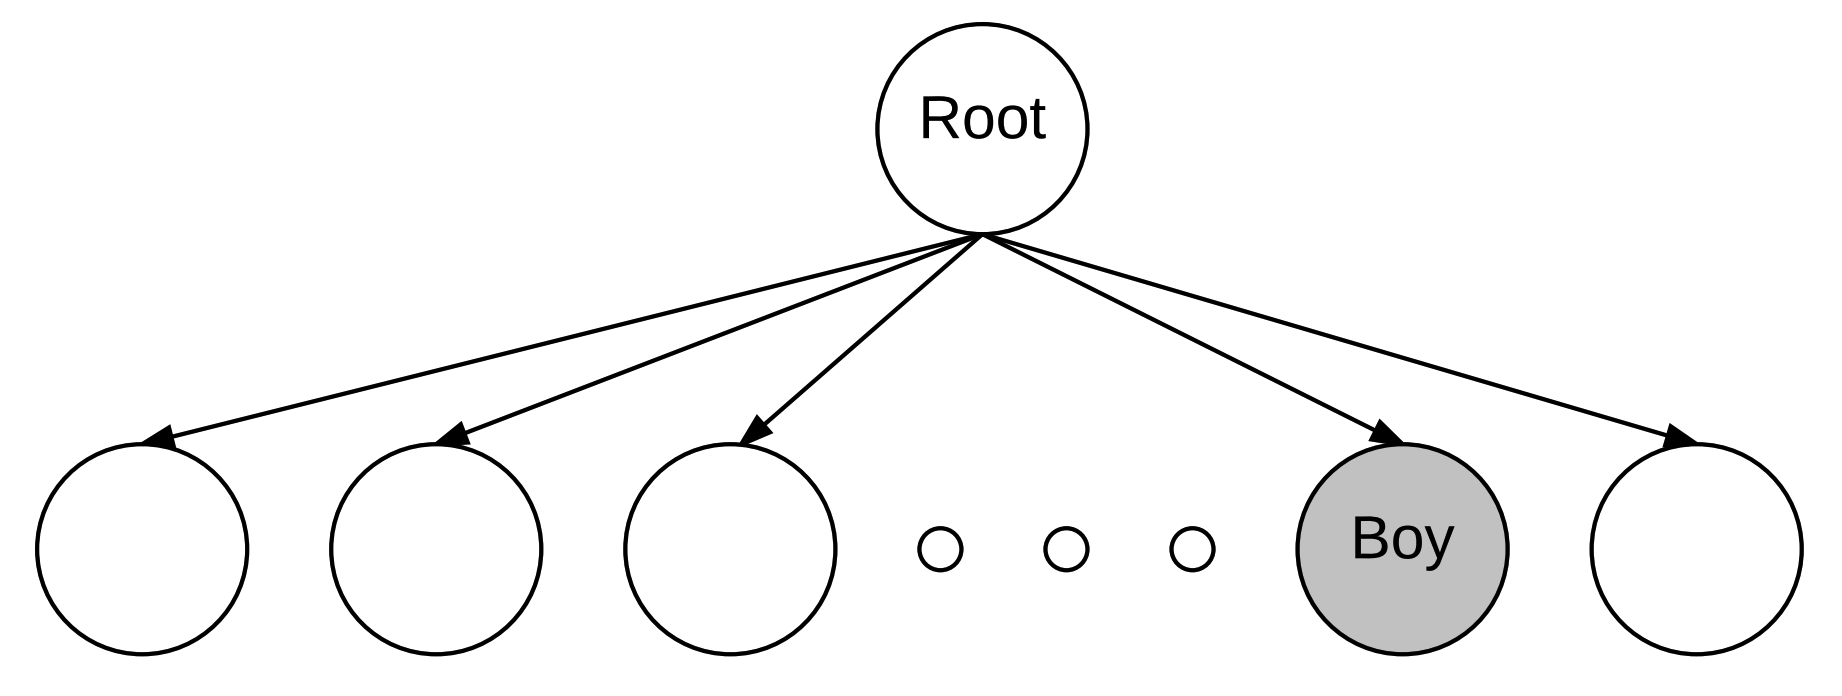
\includegraphics[width=8cm]{figs/chap4/original_nnlm.png}
		\captionsetup{justification=centering}
                \caption{Original vocabulary as flat list.\\ \color{white}{ here's the hid}}
                \label{fig:chap4:original_nnlm}
        \end{subfigure}%
        ~ %add desired spacing between images, e. g. ~, \quad, \qquad, \hfill etc.
          %(or a blank line to force the subfigure onto a new line)
        \begin{subfigure}[b]{7cm}
                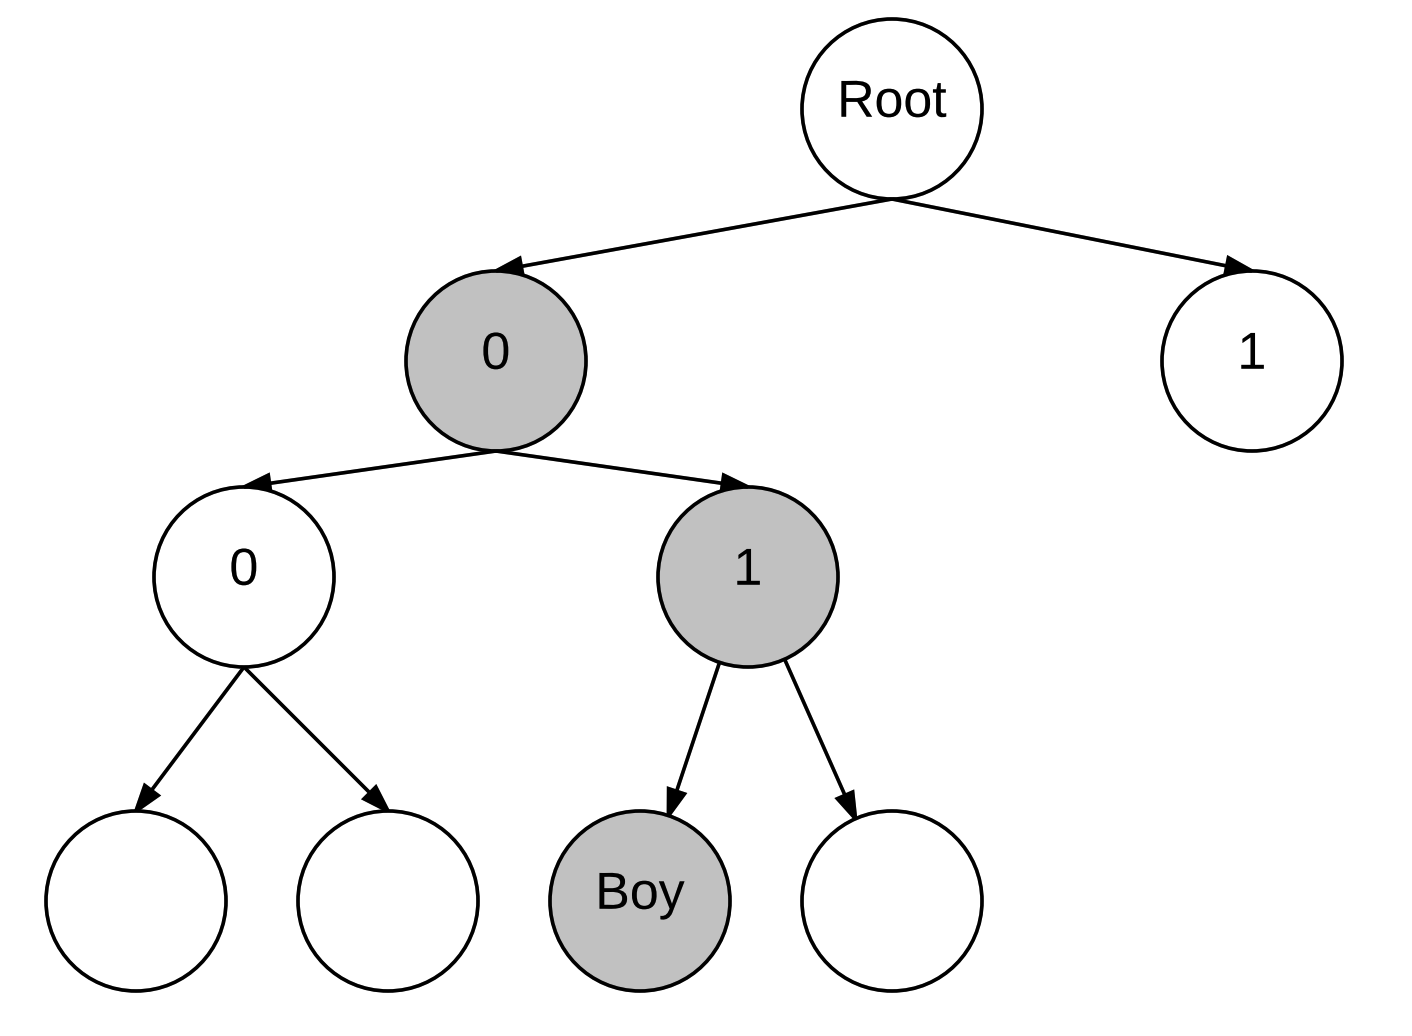
\includegraphics[width=7cm]{figs/chap4/hierarchical.png}
                \captionsetup{justification=centering}
                \caption{Binary tree vocabulary with hierarchical softmax.}
                \label{fig:chap4:hierarchical}
        \end{subfigure}
	\captionsetup{justification=centering}
        \caption[Vocabulary structures.]{Vocabulary structures of orignal neural network language model and hierarchical sampling.}
        \label{fig:chap4:vocab}
\end{figure}        

\tb{Vocabulary}

For the binary encoding of words, an optimal prefix code known as the Huffman encoding scheme was chosen~\cite{huffman52}. Constructing a Huffman binary tree starts by sorting all words by their frequency, making the two least frequent words into leaf nodes. Then their parent node is created with the sum of its children's frequencies as its frequency. Excluding the two leaves (but including their parent node), two least frequent words are again selected, and the process is repeated until a single root note remains with the sum of every word's frequency. 
\nl
I first constructed a Huffman binary encoding of every vocabulary word, then built a binary tree structure based on the encoding, as in Figure~\ref{fig:chap4:hierarchical}. Then, each bit of the Huffman embedding of a word represents a `left or right' decision in the tree, which when combined in series ultimately forms the semantic representation of the word.

\tb{Network Architecture}

\begin{figure}[htbp]
    \hspace{-2.7cm}
    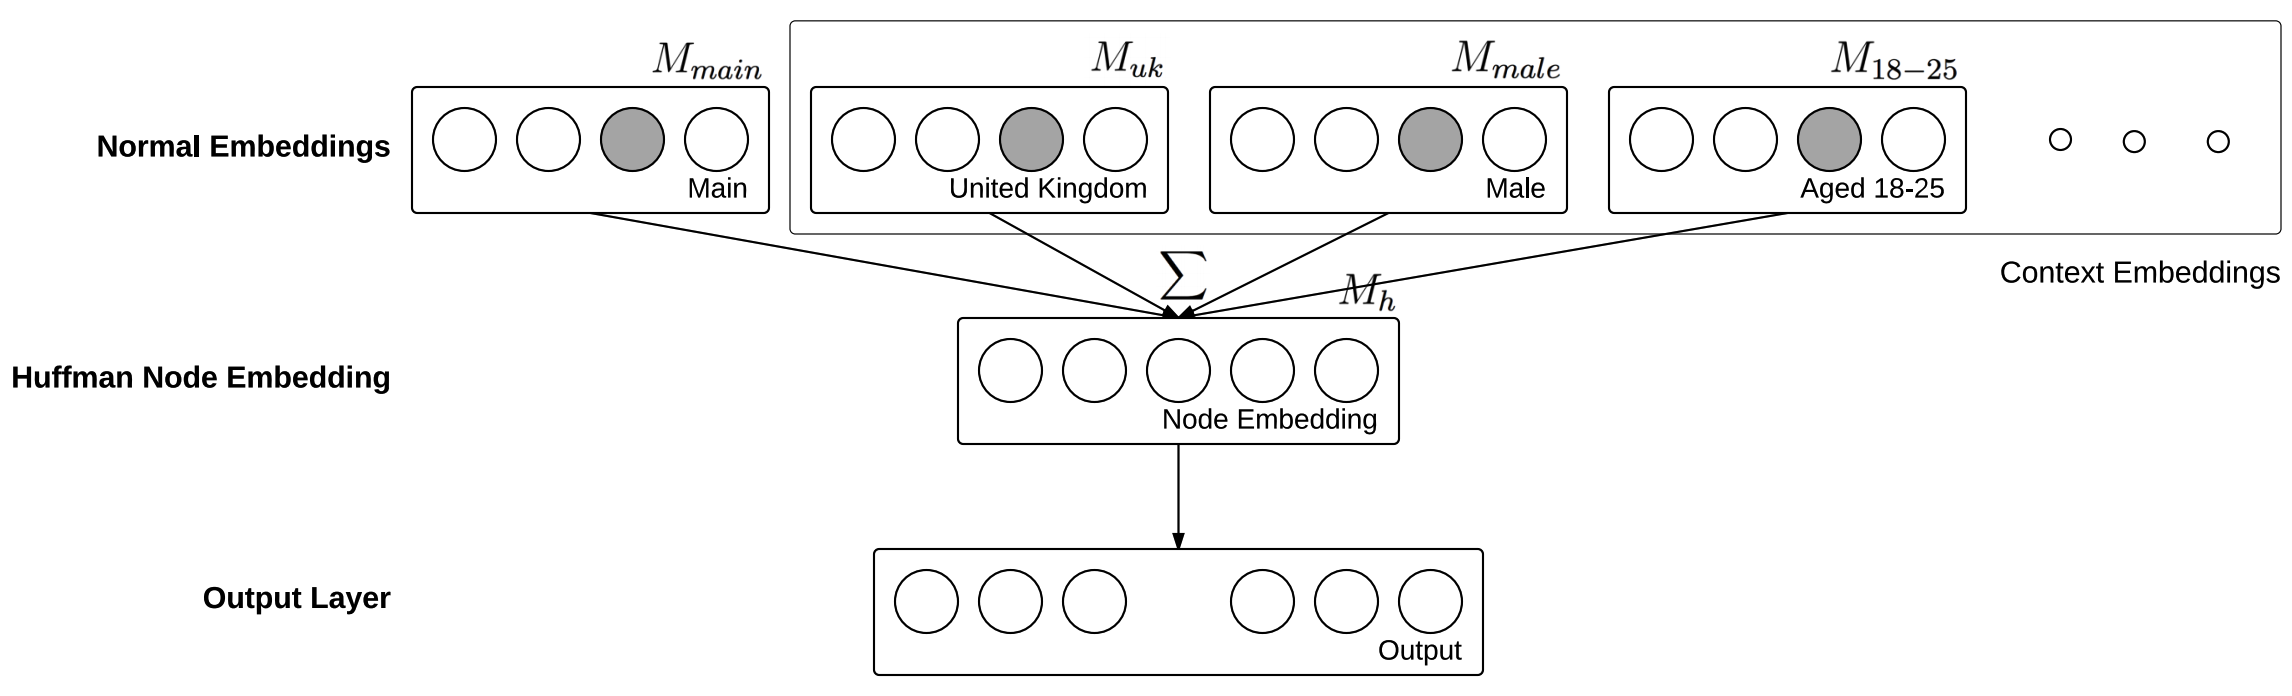
\includegraphics[width=20cm]{figs/chap4/architecture.png}
    \captionsetup{justification=centering}
    \caption[Skip-gram network architecture. ]{Skip-gram network architecture. Given an input words and its contexts, corresponding rows are accessed from the main embedding matrix $M_{main}$ and appropriate context embeddings matrices $M_c$, and summed in the hidden layer.}
    \label{fig:chap4:skipgram}
\end{figure}

Figure~\ref{fig:chap4:skipgram} shows the architecture of the context-dependent skip-gram. It has three sets of parameters (or \ti{weights} in the neural network literature): main word embeddings, context word embeddings and Huffman node embeddings. Main word embedding is a matrix $M_{main} \in \mathbb{R}^{|V|\times k}$ whose $i$-th row contains a $k$-dimensional vector for the $i$-th word in the vocabulary. An embedding for a particular word can be accessed with a \ti{one-hot vector}: $o'=(0,0,0,\dots,1,\dots,0,0,0)^{\intercal} \in \mathbb{R}^{|V|\times 1}$ as $w'={M_{main}}^{\intercal}\;o'\in \mathbb{R}^{k\times 1}.$
\nl
Context embeddings $M_{c}$ are of the same dimension as $M_{main}$ but contain word embeddings particular to a certain user context $c$ that, when combined with the main word embedding, produces final word embeddings for that context. Hence, the embedding of the word \ti{boy} for male in the US is obtained as:
$$w_{boy}'=(M_{main}+M_{male}+M_{us})^{\intercal}\;o_{boy}'$$
The Huffman node embedding matrix $M_{h} \in \mathbb{R}^{Z\times k}$ contains $k$-dimensional embeddings for each inner node in the Huffman vocabulary tree. With input and output words $w_I$ and $w_O$, and a given node level $j$ of the output word, the network computes ${v'_{n(w_O,j)}}^{\intercal}\:v_{w_I}$ as output. Note that $v_{w_I}$ is the embedding for word $w_I$ in the main word embedding matrix $M_{main}$, whereas $v'_{n(w_O,j)}$ is the Huffman node embedding for node $n(w_O,j)$ in the node embedding matrix $M_{h}$.
\refs{HOW MANY CONTEXTS HAVE BEEN CREATED}

\tb{Regularisation}

Hinton \ti{et al.} developed a biologically-inspired regularisation technique to avoid co-adaptation of weights in neural networks~\cite{hinton12}. This technique, known as \ti{Dropout}, randomly omits a hidden unit (sets to zero) from the network with some probability $p$. This is amounts to taking an average of an exponential number of different networks in a very efficient manner, as well as preventing a hidden unit from rely on the presence of any other.
\nl
Dropout was implemented in the CDSG model by randomly excluding some weights during computation of the dot product at the output layer.

\section{Training}

The model was trained using stochastic gradient ascent and backpropagation. Every training example was only fed into the network once and the weights were updated after each example. Only a small number of parameters are updated after the network sees each example: assuming the sentence has contexts \ti{US} and \ti{female}, only two rows of dimension $1\times 200$ in matrices $M_{main}, M_{us}, M_{female}$ and $M_{h}$ are updated for each ($w_I, w_O$) pair.

\tb{Objective function derivation}

The training objective of the model is to find the set of embeddings that maximises the average log probability of the training data:
\begin{equation}
\frac{1}{T}\sum_{t=1}^{T}\sum_{-c \le j \le c, j \ne 0}^{}{\log p(w_{t+j}|w_t)},
\label{eq:ch4:obj}
\end{equation}
where $T$ is the size of the training corpus. Recall that $\log p(w_{t+j}|w_t)$ in the context of skip-gram is given in Equation~\ref{eq:ch4:morin} and repeated below:
\begin{equation}
\prod_{j=1}^{L(w)-1}\sigma([\![n(w,j+1)=ch(n(w,j))]\!]\cdot {v'_{n(w,j)}}^{\intercal} v_{w_I} ).
\label{eq:ch4:sigma}
\end{equation}
Let $sim={v'_{n(w,j)}}^{\intercal} v_{w_I}$ and $code=n(w,j+1)$ (in bits, hence either 0 or 1; 0 represents the left child, while 1 represents the right). Then the expression inside the product can be re-written as:
\begin{equation}
\sigma_{obj}(code,sim)=\frac{\exp((1-code)sim)}{1+\exp(sim)}.
\label{eq:ch4:sol}
\end{equation}
The above holds because in the case where $code=0$ (\ti{i.e.} $j+1$\textsuperscript{th} node is the left child of the $j$-th node):
$$\sigma_{obj}(0,sim)=\frac{\exp(sim)}{1+\exp(sim)}=\frac{1}{1+\exp(-sim)}=\sigma(sim).$$
The expression within $[\![ \cdot]\!]$ in Equation~\ref{eq:ch4:sigma} is true because we choose $ch(n)$ to be the left child of node $n$. Consequently, it evaluates to 1. If, on the other hand, $code=1$:
$$\sigma_{obj}(1,sim)=\frac{1}{1+\exp(sim)}=\sigma(-sim).$$
The expression $[\![ \cdot]\!]$ in this case evaluates to $-1$. Note that $\sigma_{obj}(0,sim)+\sigma_{obj}(1,sim)=1, \: \forall{sim}.$
\nl
Taking the logarithm of Equation~\ref{eq:ch4:sol}, we get
$$\log\sigma_{obj}(code,sim)=(1-code)sim-\log({1+\exp(sim)}).$$
If we take its derivative with respect to $sim$,
\begin{equation}
\begin{split}
\frac{d(\log\sigma_{obj}(code,sim))}{dsim}&=1-code-\frac{\exp(sim)}{1+\exp(sim)} \\ 
									&=1-code-\sigma(sim).
\end{split}
\label{eq:ch4:code}
\end{equation}

As $sim={v'_{n(w,j)}}^{\intercal} v_{w_I}$, where $v'_{n(w,j)}={M_h}^\intercal\:o'_{w_O}$ and $v_{w_I} = (M_{main}+\sum_{c}^{}{M_{c}})^\intercal\:o'_{w_I}$ (where $o'_{w_I}, o'_{w_O}$ are one-hot vector to index into words $w_I$ and $w_O$ respectively), the derivative of $sim$ with respect to each element of the weights are:
\begin{equation}
\frac{dsim}{dM_{main}(i,j)}=\sum_{k}^{}M_{h}(k,j)
\label{eq:ch4:dmain}
\end{equation}
\begin{equation}
\frac{dsim}{dM_{c}(i,j)}=\sum_{k}^{}M_{h}(k,j).
\label{eq:ch4:dc}
\end{equation} assuming $i$ is the index of $w_I$ and $k$ ranges over the indexes of the nodes of $w_O$. $M_{main}(i,j)$ accesses the element of $i$-th row and $j$-th column in matrix $M_{main}$. Also,
\begin{equation}
\frac{dsim}{dM_{h}(k,j)}=(M_{main}+\sum_{c}^{}{M_{c}})(i,j).
\label{eq:ch4:dh}
\end{equation}

\tb{Gradient ascent}

Gradient ascent algorithm increments the parameters with the gradient of the objective function with respect to the parameter, multiplied by the learning rate. This updates the parameters in the direction of the steepest gradient.
$$\theta \leftarrow \theta + \eta\frac{\partial f_{obj}(\theta)}{\partial\theta}.$$ This can be rewritten into 
$$\theta \leftarrow \theta + \eta\frac{\partial sim}{\partial\theta}\:\frac{\partial f_{obj}(sim)}{\partial sim}.$$
Note that the latter partial derivative is given in Equation~\ref{eq:ch4:code}. Hence, this gives
\begin{equation}
\theta \leftarrow \theta + \eta\frac{\partial sim}{\partial\theta}\:(1-code-\sigma(sim)).
\label{eq:ch4:grad}
\end{equation}
Letting $\theta=M_{z}(i,j)$ where $z \in \{main,c,h\}$ , the appropriate gradient $\frac{\partial sim}{\partial M_z(i,j)}$ is given in \cref{eq:ch4:dmain,eq:ch4:dc,eq:ch4:dh}.

\tb{Backpropagation}

Standard backpropagation is performed to update the weights of the network. In forward propagation, a single row in $M_{main}$ and $M_{c}$ interacts with multiple rows in $M_h$, as the output word is decomposed into several nodes. Hence, the gradient of $M_{main}$ and $M_c$ is accumulated over all nodes on the path to the output word and updated at the end. On the other hand, each row of $M_h$ interacts only with one row of $M_{main}$ and each of $M_c$, hence can be updated immediately.

\vspace{5pt}
\begin{algorithm}[htbp]
\begin{description}
	\item For each inner node along to path to the output word $w_O$:
		\item \quad Compute a forward pass through the network, obtain $1-code-\sigma(sim).$
		\item \quad Update $M_{h}$ with the gradient of $M_h$: sum of relevant rows in $M_{main}$ and $M_c$.
		\item \quad Accumulate gradients of $M_{main}$ and $M_c$.		
	\item Update $M_{main}$ and $M_c$ with the accumulated gradient.
\end{description}
\caption{Outline of training process.}
\label{alg:chap4:backprop}
\end{algorithm}

\tb{Context-specific learning rate}

Mikolov's implementation uses a single global learning rate that linearly decays from an initial value. All weights in $M_{main}$ and $M_h$ are updated with the same learning rate. 
\nl
For the context-dependent skip-gram, given that examples with different contexts appear with different frequencies in the training data, it makes sense to have a separate learning rate for each context $c$. This enables the network to learn relatively little from a single example of frequently occurring contexts, and to pay more attention to examples with rare and informative contexts, thereby learning more from those occurrences.
\nl
The learning rate $\eta(c,t)$ for the context $c$ at time $t$ during training evolves as:
$$ \eta(c,t) = \max(\eta_{min}, \eta_0 \times(1-\frac{\delta_t(c)}{\delta_{total}(c)})).$$
$\eta_{min}, \eta_0$ are predefined values for initial and final learning rates (shared by all contexts). $\delta_t(c)$ is the number of words associated with context $c$ seen so far up to time $t$ during training, and $\delta_{total}(c)$ is the total number of words tagged with context $c$ in the training corpus. Empirically, $\eta_{min}, \eta_0$ were chosen as $0.0001$ and $0.1$.

\section{Implementation}

\tb{Cython}

Rehurek's implementation was optimised for selected hotspots by calling core C routines and BLAS functions within Cython code. As Cython's memory management is not thread-safe, implementing training and dropout in Cython involved careful use of global mutex called GIL (Global Interpreter Lock) to prevent several threads from accessing Python bytecodes simultaneously.

\vspace{0.3cm}
\begin{lstlisting}[language=Python,caption={Cython code for dropout regularisation at the hidden layer.},label=lst:chap4:dropout]
for a in range(0, size):
    syntemp[a] = syn0[indexes[j] * size + a]

# Summing context embeddings 
for x in range(0, context_length):
    for a in range(0, size):
        syntemp[a] += syncon[ (contexts[x]*vocab_size*size)
        						 + indexes[j] * size + a ]

# Dropout
for a in range(0, size):
    if (xor32() % 100) < dropout_param:
        syntemp[a] = 0
\end{lstlisting}

Listing~\ref{lst:chap4:dropout} shows a Cython code snippet to implement summation of main and context word embeddings at the input layer and drop hidden units out with some probability afterwards.

\tb{BLAS functions}

BLAS (Basic Libear Algebra Subprograms) is a set of interfaces to perform linear algebra operations with heavy optimisations in C and Fortran. As several operations in the backpropagation routine involve computing the dot product of vectors, BLAS functions were used to optimise a loop of similar linear algebra operations. An example is the \tx{dsdot(n,x,incx,y,incy)} function, which computes the dot product of vectors \tx{x} and \tx{y} of size \tx{n}, with increment \tx{incx} and \tx{incy} to index each element of the vectors.

\tb{Precomputed sigmoid table}\footnote{Optimisation used by Mikolov \ti{et al.} in the C implementation: \url{https://code.google.com/p/word2vec/source/browse/trunk/word2vec.c}.}

As Equation~\ref{eq:ch4:grad} shows, computing the gradient involves obtaining $\sigma(sim)$. As evaluating the sigmoid function on every training example can lead to a significant performance hold-up, the sigmoid function was precomputed in discretised steps and stored in a table, effectively replacing explicit sigmoid evaluations in the core training routine with dictionary lookups.

\begin{lstlisting}[language=Python,caption={Cython code for precomputing and accessing sigmoid function.},label=lst:chap4:sigmoid]
# computing the sigmoid table.
for i in range(SIG_TABLE_SIZE):
	SIG_TABLE[i] = exp((i / SIG_TABLE_SIZE * 2 - 1) * MAX_SIG)
	SIG_TABLE[i] = (SIG_TABLE[i] / (SIG_TABLE[i] + 1))

# f is the vector similarity (dot product)
if f <= -MAX_SIG or f >= MAX_SIG:
	continue
f = SIG_TABLE[((f + MAX_SIG) * (SIG_TABLE_SIZE / MAX_SIG / 2))]
\end{lstlisting}

\begin{figure}[htbp]
%   \vspace{-1.5cm}
   \centering
    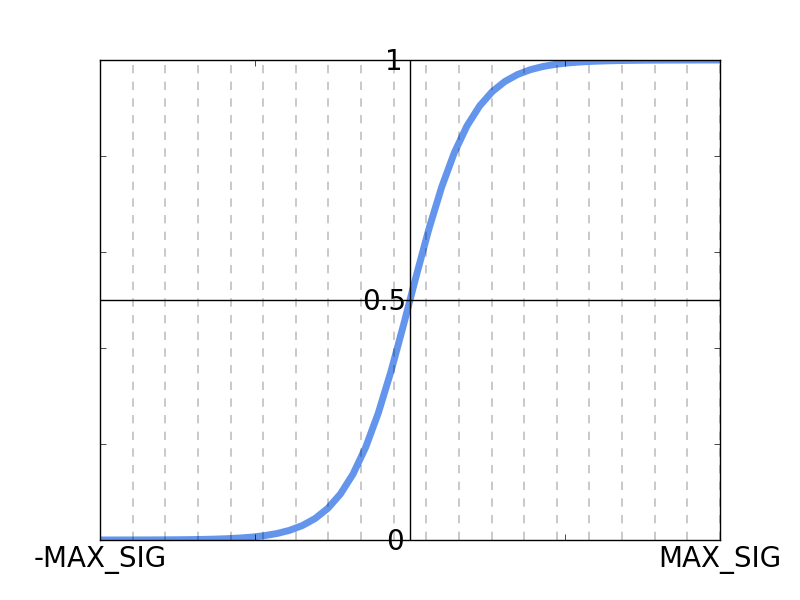
\includegraphics[width=9cm]{figs/chap4/sigmoid.png}
    \captionsetup{justification=centering}
    \caption[Discretisation of the sigmoid function. ]{The sigmoid function is discretised into \tx{SIG\_TABLE\_SIZE} pieces.}
    \label{fig:chap4:sigmoid}
%    \vspace{-1cm}
\end{figure}

In Figure~\ref{fig:chap4:sigmoid}, note that $\sigma(x)\approx 1$ if $x$ is large and $\sigma(x)\approx 0$ if $x$ is small. Hence we define a boundary \tx{MAX\_SIG} such that we approximate the function as 0 and 1 if $x$ is beyond either barrier. Within that range, we discretise the function into \tx{SIG\_TABLE\_SIZE} pieces. Concretely, \tx{MAX\_SIG} and \tx{SIG\_TABLE\_SIZE} were chosen to be 6 and 1000, respectively. 
\nl
In Listing~\ref{lst:chap4:sigmoid}, \tx{SIG\_TABLE} is defined as:
\begin{equation}
\begin{split}
\tx{SIG\_TABLE[i]} &= \frac{ \exp((\frac{2*i}{\tx{SIG\_TABLE\_SIZE}} - 1) * \tx{MAX\_SIG}) }{\exp((\frac{2*i}{\tx{SIG\_TABLE\_SIZE}}  - 1) * \tx{MAX\_SIG}) + 1} \\
				&= \frac{1}{1+\exp(-(\frac{2*\tx{MAX\_SIG}}{\tx{SIG\_TABLE\_SIZE}}*i - \tx{MAX\_SIG}) )}
\end{split}
\end{equation}

Then, 
%\begin{multline}
$$\tx{SIG\_TABLE}[((f + \tx{MAX\_SIG}) * \frac{\tx{SIG\_TABLE\_SIZE}}{\tx{MAX\_SIG}*2})] $$
\begin{equation}
\begin{split}
&= \frac{1}{1+\exp(-(\frac{2*\tx{MAX\_SIG}}{\tx{SIG\_TABLE\_SIZE}}*((f + \tx{MAX\_SIG}) * \frac{\tx{SIG\_TABLE\_SIZE}}{\tx{MAX\_SIG}*2}) - \tx{MAX\_SIG}) )} \\
&= \frac{1}{1+\exp(-((f + \tx{MAX\_SIG}) - \tx{MAX\_SIG}) )} \\
&= \frac{1}{1+\exp(-f)} \\
&= \sigma(f)
\end{split}
\end{equation}
%\end{multline}

Hence, this method correctly computes the value of the sigmoid function.

\tb{Shuffling tweets}

As that the learning rate decreases linearly throughout training, the network learns the most from examples that appear early in the training corpus. Therefore, shuffling the order of the tweets causes huge perturbations on the evolution of the cost function of the network, thereby allowing the model to explore different regions of the cost surface throughout several iterations of training. When training the same model several times to obtain the performance bound, the examples were shuffled by random for each training session. This leads to a more robust evaluation of the model's performance independently of the order of samples. 

\tb{Initialising embeddings}

Mikolov's implementation of Skip-gram initialises each element of the general embedding matrix with a random draw from a uniform distribution $[-0.5, 0.5].$ This is the only source of randomness in the original C implementation. However, I chose to initialise the general embeddings with an external embedding matrix pre-learnt from a standard corpus such as Wikipedia. This will potentially lead to performance improvements because the model now has substantial knowledge about facts from Wikipedia. For example, it can now learn more nuanced changes in meaning of `Mercedes' in different contexts as it already knows that Mercedes is a carmaker. 
\nl 
As such, I trained the standard Skip-gram model on the first billion characters from Wikipedia\footnote{\url{http://mattmahoney.net/dc/enwik9.zip}}. Then, I initialised the general embeddings of words in my model with the embeddings learnt from Wikipedia. The words in my model that do not occur in Wikipedia were simply initialised as before: uniformly distributed as $[-0.5,0.5].$

\section{Measuring brand perception}

Word association in the vector space model is commonly measured with \ti{cosine similarity} between the two word vectors. Once the context-dependent model is trained, its word embeddings change for different contexts. I propose to measure brand perception as the cosine similarity between word embeddings that represent product category and brand names. For example, to see which of \ti{smirnov, absolut} and \ti{svedka} is most associated with \ti{vodka}, I compute the following:
$$ sim(x,vodka), \: x \in \{smirnov, absolut, svedka\}.$$
$sim(a,b)$ is the cosine similarity between $vec(a)$ and $vec(b)$. The item with the greatest cosine similarity with \ti{vodka} is the one most associated with vodka according to the model's learnt embeddings.
\\ \\
On the other hand, to measure perception with contexts, I can instead compute:
$$ sim_{x}(alcohol,beer), \: x \in \{male, female\},$$
where $sim_{c}(a,b)$ denotes the cosine similarity between $vec(a)$ and $vec(b)$ in the context of $c$. Computing this first involves adding context embeddings for $c$ to the main embeddings of $a$ and $b$, \ti{i.e.}
$$ sim_{c}(a,b) = sim(vec_{main}(a)+vec_c(a),vec_{main}(b)+vec_c(b)).$$
Beer can be said to be more associated with alcohol for one gender if the similarity between $vec(beer)$ and $vec(alcohol)$ is greater in the context of that gender. 

%% EVALUATION

\chapter{Evaluation} 
\label{ch5}

\section{Evaluation setting}

This chapter evaluates the effectiveness of the context-dependent skip-gram model by comparatively assessing the quality of context embeddings against those learnt by a model insensitive to user contexts. Then, it presents notable observations of context embeddings' ability to capture various contextual variations of word meanings.

\tb{Models}

In quantative evaluation schemes (see Section~\ref{ch5:2}), three models were evaluated against each other: 
\begin{itemize}[itemsep=-5pt]
	\item SGLM: Mikolov's vanilla Skip-gram model augmented with context embeddings.
	\item CDSG: SGLM model with context-specific learning rates.
	\item CDSGD: CDSG model with 10\% of its hidden units randomly omitted with dropout. 10\% was found to give best performance.
\end{itemize}

\tb{Parameter set}

The list of model-generic parameters and the values used in practice are given below:

\begin{itemize}[itemsep=-5pt]
	\item vector\_size : the dimension of the learned vector representations, chosen to be 200.
	\item ini\_alpha : initial learning rate (both general and context-specific), chosen to be 0.1. 
	\item min\_alpha : minimum learning rate (both general and context-specific), chosen to be 0.0001.
	\item window : the width of the context-window from which to perform word prediction, chosen to be 5. This implies that all contexts within five words to the left and the right were used to predict the current word.
	\item min\_count : the threshold for which words appearing in corpus with a smaller frequency are ommitted, chosen as 50.
\end{itemize}

\section{Quantitative evaluation}
\label{ch5:2}

As a quantitative measure of the model's ability to learn context-sensitive representations of language, I constructed three different evaluation schemes, which each test if the model captures different types of metadata well.

\subsection{Location}

\tb{Dataset and methodology}

To evaluate the accuracy of geographic embeddings, I adopted the dataset used by Bamman \ti{et al.} to evaluate distributed representations to learn geographically situated language~\cite{bamman14}. The authors measure semantic similarity of pairs of words whose meaning has strong geographic correlations and report the mean similarity of geographically-related pairs of words. For example, in U.S., California, we expect the word \ti{state} to be associated most with \ti{california} than any other American state, such as \ti{texas}. I take the rank of \ti{california} from all states based on the similarity to vector \ti{state} in the context of \ti{california}, and proceed with other states analogously. Six categories of words with strong geographic connotation were constructed, as shown below. For each category, an example of the list of similarities to be computed is shown for each sports team/state, with the target similarity (the one we expect to rank highest) displayed in bold.

\begin{enumerate}[itemsep=-15pt]
	\item \tb{state}: for each state, I compute the similarity between the word \ti{state} and every US state, in the context of that state; \\ \ti{e.g.}, $\mathbf{sim_{CA}(state,california)},sim_{CA}(state, texas),sim_{CA}(state, arizona),\\ \cdots$ for the state California.
	\item \tb{city}: for each state, I compute thet similarity between the word \ti{city} and the most populous city of each state, in the context of that state; \ti{e.g.}, $\mathbf{sim_{MA}(city,boston)},sim_{MA}(city,new\:york), sim_{MA}(city,houston),\\ \cdots$ for the state Massachusetts. 
	\item \tb{basketball}: for each NBA team, I compute the similarity between $(vec(basketball)+vec(team))$ and every NBA team name, in the context of the state the team is based in; \\ \ti{e.g.} $\mathbf{sim_{IL}(basketball+team,bulls)},sim_{IL}(basketball+team,knicks),\\sim_{IL}(basketball+team,celtics), \cdots$ for the team Chicago Bulls
	\item \tb{baseball}: for each MLB team, I compute the similarity between \\ $(vec(baseball)+vec(team))$ and every MLB team name, in the context of the state the team is based in; \\ \ti{e.g.} $\mathbf{sim_{MA}(baseball+team,red\:sox)},sim_{MA}(baseball+team,yankees),\\sim_{MA}(baseball+team,white\:sox),\cdots$ for the team Boston Red Sox. 
	\item \tb{football}: for each NFL team, I compute the similarity between \\ $(vec(football)+vec(team))$ and every NFL team name, in the context of the state the team is based in; \\ \ti{e.g.} $\mathbf{sim_{TX}(football+team,cowboys)},sim_{TX}(football+team,giants),\\ sim_{TX}(football+team,bears),\cdots$ for the team Dallas Cowboys.
	\item \tb{hockey}: for each NHL team, I compute the similarity between \\ $(vec(hockey)+vec(team))$ and every NHL team name, in the context of the state the team is based in;\\  \ti{e.g.} $\mathbf{sim_{NJ}(hockey+team,devils)},sim_{NJ}(hockey+team,rangers),\\ sim_{NJ}(hockey+team,islanders),\cdots$ for the team New Jersey Devils.
\end{enumerate}

\begin{figure}[htbp]
	\hspace{-2.3cm}
        \begin{subfigure}[b]{9cm}
                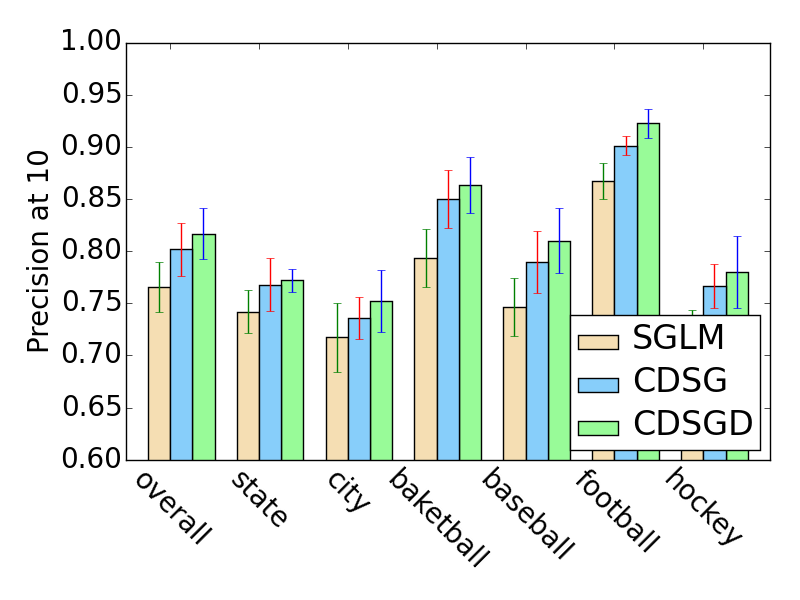
\includegraphics[width=9cm]{figs/chap5/loc_prec.png}
                \caption{Precision at 10 for each category}
                \label{fig:chap5:loc_prec}
        \end{subfigure}%
        ~ %add desired spacing between images, e. g. ~, \quad, \qquad, \hfill etc.
          %(or a blank line to force the subfigure onto a new line)
        \begin{subfigure}[b]{9cm}
                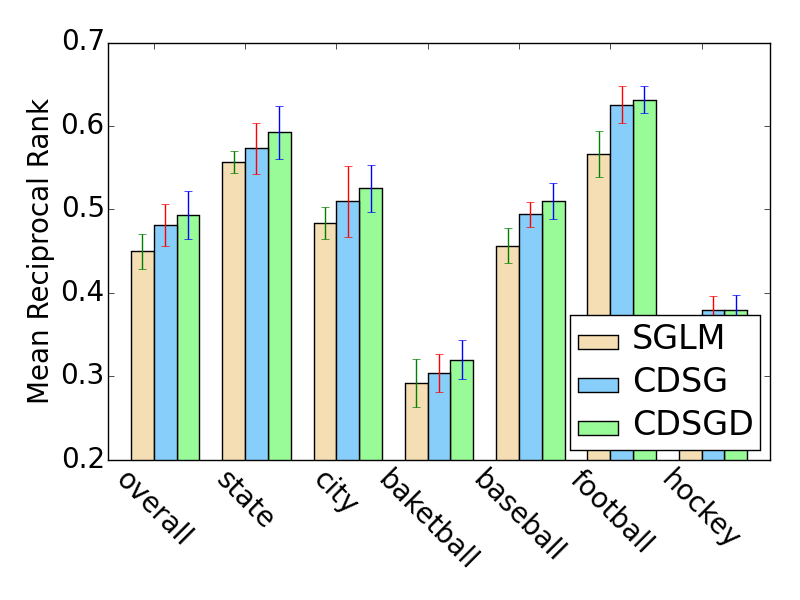
\includegraphics[width=9cm]{figs/chap5/loc_mrr.png}
                \caption{Mean reciprocal rank for each category.}
                \label{fig:chap5:loc_mrr}
        \end{subfigure}
	\captionsetup{justification=centering}
        \caption[Location evaluation results.]{Location evaluation results.}
        \label{fig:chap5:loc_eval}
\end{figure}

Three models (SGLM, CDSG, CDSGS) were each run five times with the same parameter set and the training data shuffled. In Figure~\ref{fig:chap5:loc_eval}, I report the average precision at 10 and mean reciprocal rank for each category, with standard deviation for each category as an error bar. I explain both evaluation metrics below.

\begin{itemize}
	\item Precision at 10 : In California, we expect \ti{california} (current word) to be more similar to \ti{state} (target word) than any other US state names (competitor words). I report the ratio of current words that rank within the top 10 of all competitor words, based on the similarity between the target word. The precision at 10 of 0.8 implies that the expected word appears in the first 10 ranked by similarity, empirically with probability 0.8.
	\item Mean reciprocal rank : In Massachusetts, we expect \ti{red sox} to be more similar to \ti{baseball}+\ti{team} then other MLB team names. I report the mean of the inverse of the rank of the current word (\ti{red sox}) amongst all competitor words. An average MRR of 0.5 implies that the expected word appears in the first 2 names returned.
\end{itemize}

\tb{Results}

Figure~\ref{fig:chap5:loc_eval} presents the result of location evaluation with two metrics, with 95\% confidence interval shown as error bars. It is clear that context-dependent models learn more accurate geographic embeddings than the vanilla skip-gram model in general. Specifically, CDSG with dropout attained 81.6\% precision at 10 on average, while the context-independent model gave 76.6\%. The difference between the two models is over 4\% for mean reciprocal rank. This demonstrates that a model with a separate learning rate for each context is able to achieve local optimum in the cost space more often and obtain better quality context embeddings.
\nl
As a concrete example, after running the CDSG model with dropout, the word \ti{texas} was the closest word in the vocabulary of 1,521,103 words to the word \ti{state} in the context of Texas, with similarity 0.770. For the CDSG model, however, the cosine similarity was 0.596 (rank \#10). For the skip-gram model, \ti{texas} was the 18\textsuperscript{th} most similar word to \ti{state}, with similarity 0.512.

\subsection{Gender}

\tb{Dataset and methodology}

As a quantative measure of the model's performance with gender-specific word representations, I compiled an evaluation dataset of 24 words, 12 for each gender, that are shown to be particularly better known to members of that gender than the other (Brysbaert, 2014).\footnote{\url{http://gnodevel.ugent.be/crr.ugent.be/archives/1628}}
\\ \\
Table~\ref{tab:chap5:gender} shows top 12 recognisable words for each gender in column `Word1'. The column `Rate' shows the recognition rates: $(a, b)$ signifies that $a$ percentage of men could correctly recognise the meaning of the word, while $b$ percentage of women could do the task. Then, column `Word2' gives a single word that is a synonym of or a generally associated word with `Word1' according to Oxford Dictionaries.\footnote{\url{http://www.oxforddictionaries.com/}}

\begin{table}[htbp]
\begin{center}
\begin{tabular}{ lll|lll }
    \multicolumn{3}{c}{Male Words}  & \multicolumn{3}{c}{Female Words}  \\ \hline
    Word1 & Rate & Word2 & Word1 & Rate & Word2 \\ \hline
    codec & (88, 48) & data & taffeta & (48, 87) & silk  \\
    solenoid & (87, 54) & coil & tresses & (61, 93) & hair \\
    golem & (89, 56) & robot & bottlebrush & (58, 89) & brush \\
    mach & (93, 63) & speed & flouncy & (55, 86) & decorative \\
    humvee & (88, 58) & vehicle & mascarpone & (60, 90)& cheese  \\
    claymore & (87, 58) & sword & decoupage & (56, 86) & paper \\
    scimitar & (86, 58) & sword & progesterone & (63, 92) & hormone\\
    kevlar & (93, 65) & fiber & wisteria & (61, 89) & pea \\
    paladin & (93, 66) & warrior & taupe & (66, 93) & grey \\
    bolshevism & (85, 60) & communism & flouncing & (67, 94) & angry \\
    biped & (86, 61) & two-footed & peony & (70, 96) & plant \\
    dreadnought & (90, 66) & battleship& bodice & (71, 96) & dress\\
    \hline
\end{tabular}
\end{center}
\caption{Gender evaluation dataset.}
\vspace{-0.1cm}
\label{tab:chap5:gender}
\end{table}

For each row in the table, I computed $\sigma_{m} = sim_{male}(vec(word1), vec(word2))$ and $\sigma_{f} = sim_{female}(vec(word1), vec(word2))$. Then, I computed the Spearman's rank correlation of the difference between male rates and female rates and ${\sigma_m} - {\sigma_f}$ for each row. Spearman's rank correlation, also known as Spearman's $\rho$, is a non-parametric metric of statistical dependence between two variables. It shows how well the relationship between the two variables can be represented using a monotonic function (not necessarily linear). A perfect Spearman correlation of +1 or -1 is achieved when the two variables are in a perfectly monotonic relationship, or its inverse. The intuition here is that for words with large recognition rate gap between genders, the similarity between `Word1' and `Word2' should also greatly differ between two genders.
\nl
For a sample size $n$, raw scores $X_i,\: Y_i$ are converted to ranks $x_i, y_i$ and $\rho$ is computed as:
$$\rho = 1-6\frac{\sum_{}^{}{{d_i}^2}}{n(n^2-1)},$$
where $d_i = x_i - y_i$, \ti{i.e.} the difference between ranks. To report the overall correlation from five independent trials, I first converted each $\rho_i$ using Fisher's z-transformation:
$$z_i = \frac{1}{2}\ln(\frac{1+\rho_i}{1-\rho_i})=\arctanh(\rho_i).$$
Then, I averaged $z_i$ as $\bar{z} = {\sum_{i=1}^{5}{z_i}}/{5}$ and backtranform the averaged $\bar{z}$ into the $\rho$ space:
$$\bar\rho = \frac{\exp(2\bar{z})-1}{\exp(2\bar{z})+1} = \tanh(\bar{z}).$$
The bottommost row in Table~\ref{tab:chap5:gender_eval} shows the overall correlation $\bar\rho$ over five trials derived as above.
\nl
As a concrete implementation of Spearman's rho, I used the \tx{spearmanr} function of package \tx{scipy.stats}. The function returns the correlation coefficient and p-value as output, where the p-value describes the chance that random sampling would result in the correlation coefficient obtained when there is no correlation between two random variables. 
\nl
As in location evaluation, three models (SGLM, CDSG, CDSGD) were trained five times each with the same set of parameters. Table~\ref{tab:chap5:gender_eval} presents the correlation coefficient and p-value for each training trial as well as the overall correlation for each model. Rows with `Word1' nonexistent in the vocabulary were dropped from computation. 

\tb{Results}

\begin{table}[h]
\centering
\begin{tabular}{lllllll}
 \multicolumn{1}{c}{}   & \multicolumn{2}{c}{SGLM} & \multicolumn{2}{c}{CDSG} & \multicolumn{2}{c}{CDSGD} \\ \cline{2-7}
        & Corr      & P-val        & Corr           & P-val             & Corr          & P-val       \\ \cline{2-7}
Trial 1 & 0.405         & 6.842E-3 &  0.463         & 3.451E-2         & 0.575     & 6.139E-4                 \\
Trial 2 & 0.562         & 8.020E-3 &  0.539         & 1.166E-3         & 0.593     & 3.778E-4                \\
Trial 3 & 0.415         & 6.141E-3 &  0.589         & 4.939E-3         & 0.603     & 3.815E-4                 \\
Trial 4 & 0.598         & 4.215E-2 &  0.622         & 2.584E-3         & 0.734     & 1.537E-4                \\
Trial 5 & 0.609         & 3.403E-4 &  0.749         & 9.265E-5         & 0.514     & 1.702E-3                 \\ \hline
\multicolumn{1}{l}{Overall}
        & 0.523         &          & 0.602          &                  & 0.609     &                    \\ \hline\end{tabular}
\caption{Gender evaluation results.}
\label{tab:chap5:gender_eval}
\end{table}

As Table~\ref{tab:chap5:gender_eval} shows, the context sensitive models perform noticeably better than the skip-gram model, a clear indication that the gender-specific embeddings learnt by the last two models are of arguably better quality than those for the context-independent model. As a concrete example, the similarity between \ti{scimitar} and \ti{word} for male was 0.250 for male and 0.087 for female under the CDSGD model. However, for the skip-gram model, the similarities were 0.211 for male and 0.213 for female. Although the number of test cases is rather small (24), each p-value of individual correlation coefficient is reasonably small ($<$4\%) to reject the null hypothesis that the purported correlation does not exist.

\subsection{General Semantic Similarity}

\tb{Dataset and methodology}

In addition to context-specific embeddings, the accuracy of general word embeddings was tested with standard word similarity tasks, using corpora WordSimilarity-353 and SimLex-999. WordSimiliarity-353 dataset contains 353 word pairs tagged with the average of their similiarity scores assigned by 13-16 subjects~\cite{finkelstein02}. The instruction to subjects was to measure the \ti{relatedness} of the pair of words on a scale from 0 (totally unrelated words) to 10 (very similar words or synonyms). SimLex-999 is a more recent dataset that provides a gold standard for word \ti{similiarity} rather than relation or association. Hill \ti{et al.} demonstrate that SimLex-999 is challenging for computational language models to capture as they should learn word similarity independently of relatedness. Most language representation learning models infer relationship between words from their co-occurrences, which primarily reflects relatedness not similarity~\cite{hill14}.

\begin{table}[h]
\centering
\begin{tabular}{lll}
           & SimLex-999 & WordSim-353 \\ \cline{2-3}
\ti{coast-shore}    & 9.00              & 9.10               \\
\ti{clothes-closet} & 1.96              & 8.00              \\ \cline{2-3}
\end{tabular}
\caption{Comparison of WordSim-353 and SimLex-999 evaluation datasets.}
\end{table}

\tb{Results}

\begin{table}[h]
\centering
\begin{tabular}{llllllll}
 &\multicolumn{1}{c}{}   & \multicolumn{2}{c}{SGLM} & \multicolumn{2}{c}{CDSG} & \multicolumn{2}{c}{CDSGD} \\ \cline{3-8}
&        & Corr      & P-val        & Corr       & P-val       & Corr        & P-val       \\ \hline
\parbox[t]{2mm}{\multirow{6}{*}{\rotatebox[origin=c]{90}{WordSim-353}}} 
& Trial 1  &  0.510           & 1.935E-23     &  0.439          & 3.775E-17  & 0.491     & 1.230E-21                      \\
& Trial 2 & 0.466            &  2.143E-19     &  0.447          & 9.341E-18  & 0.481     & 1.142E-20                     \\
& Trial 3 & 0.460            & 8.149E-19      &   0.474         &  4.483E-20 & 0.497     & 3.369E-22                     \\
& Trial 4 & 0.516            &  4.896E-24     &   0.452         &  3.599E-18 & 0.488     & 2.510E-21                     \\
& Trial 5 &0.440             & 3.540E-17      &   0.465         & 2.702E-19  & 0.490     & 1.514E-21                     \\ \cline{3-8}
& \multicolumn{1}{l}{Overall}
           & 0.479            &              & 0.456           &             & 0.490     &                     \\ \hline
\parbox[t]{2mm}{\multirow{6}{*}{\rotatebox[origin=c]{90}{SimLex-999}}} 
& Trial 1 & 0.232     & 1.213E-13     &  0.178          & 1.477E-08             &  0.214           & 8.055E-12            \\
& Trial 2 & 0.209     & 2.454E-11     &  0.216          & 6.231E-12            & 0.223            &  1.047E-12           \\
&Trial 3 & 0.187     & 2.652E-09     &   0.232         &  1.083E-13           & 0.194            & 6.943E-10            \\
& Trial 4 & 0.217     & 4.676E-12     &   0.200         &  1.940E-10           & 0.186            &  3.027E-09           \\
& Trial 5 & 0.212     & 1.406E-11     &   0.195         & 5.874E-10            &0.198             & 3.219E-10            \\ \cline{3-8}
& \multicolumn{1}{l}{Overall} & 0.212     &              & 0.204           &             & 0.203            &           \\ \hline
\end{tabular}
\caption{General semantic similarity results.}
\label{tab:chap5:sem_sim}
\end{table}

The correlation coefficients obtained confirm that SimLex-999 is indeed more difficult for computational models to capture than WordSim-353. However, no one model was shown to learn better quality general word embeddings than the other two. On WordSim-353, CDSGD model gave the biggest correlation with the gold-standard, despite with marginal difference with the other models. On SimLex-999, however, it gave the worst performance, again with minor differences. 
\\ \\
In terms of how models are designed, there is no reason to believe that one model should learn better general word representations than any other, as all three models use the same training algorithm to backpropagate errors to update the general embeddings. As a result, I conclude there is no clear winner for the two general word semantic similarity tasks.

\section{Qualitative evaluation}

Table~\ref{tab:chap5:reverse_dic} presents the closest terms to \ti{cheers} in both UK and US after running the CDSGD model. It clearly demonstrates that the word cheers strongly evokes the sense of drinking in the US, as its close terms are either types of alcohol or related to the act of drinking. In the UK, however, the meaning of cheers seems to be more diverse, ranging from a parting wish (\ti{e.g.} \ti{xx}) or an expression of gratitude to someone close (co-occurs with \ti{e.g. name, mate, friends, brother}).

\begin{table}[h]
\centering
\begin{tabular}{ll|ll}
\multicolumn{2}{c}{US} & \multicolumn{2}{c}{UK} \\ \hline
term             & cosine            & term              & cosine              \\ \hline
cheers          & 1.000                  & cheers                  & 1.000                    \\
\#beer                 & 0.538                  & name                  & 0.584                    \\
\#craftbeer                 & 0.515                  & well                  & 0.573                    \\
kolsch                 & 0.499                  & xx                  & 0.568                    \\
brewery                 & 0.497                  & pal                  & 0.547                    \\
\#happyhour                 & 0.487                  & lads                  & 0.546                    \\
ipa                 & 0.448                  & mate                  & 0.525                    \\
gose                 & 0.445                  & friends                  & 0.520                    \\
root                 & 0.445                  & \#beer                  & 0.520                    \\
fest                 & 0.443                  & brother                  & 0.513                   \\ \hline                 
\end{tabular}
\caption{Terms with the biggest cosine similarity to \ti{cheers} for people in US/UK}
\label{tab:chap5:reverse_dic}
\end{table}

Table~\ref{tab:chap5:reverse_dic_age} shows an interesting variation of the meaning of \ti{work} based on speaker's age. The list of close terms for people aged 18 or less exhibits a strong correlation to studying, homework and school. For the next age group, the meaning gradually shifts to professional work, mirrored by terms \ti{pay} and \ti{money}. This becomes more pronounced in the last age group, for which the amount of training data is relatively small, a possible explanation for the small similarity values.
\\ \\
Given that a language model computes the sense of `similarity' based on the co-occurrence of two words, some results are not directly similar to work but related, for example \ti{hand} as in a student handing in work. The results are interesting because they not only reveal similar terms for each age group but also capture words that portray and mark each period of one's life.

\begin{table}[h]
\centering
\begin{tabular}{ll|ll|ll}
\multicolumn{2}{c}{$<18$} & \multicolumn{2}{c}{$18-25$} & \multicolumn{2}{c}{$> 25$} \\ \hline
term             & cosine            & term              & cosine          & term              & cosine              \\ \hline
work          & 1.000                  & work                  & 1.000  & work & 1.000                   \\
hard                 & 0.722                  & stuff                  & 0.791          & make & 0.457          \\
class                 & 0.719                  & home                  & 0.779         &car & 0.435           \\
probably                 & 0.697                  & money                  & 0.763          & home & 0.428          \\
stuff                 & 0.689                  & drive                  & 0.754          & pay & 0.396          \\
friends                 & 0.688                  & life                  & 0.741        &budget&0.391            \\
school                 & 0.652                  & class                  & 0.737       &drive&0.388             \\
hand                 & 0.651                  & drinks                  & 0.736          &money&0.383          \\
college                 & 0.642                  &  sleep                 &   0.730    &commute&0.333              \\
questions                 & 0.641                  & pay                  & 0.724        &kids&0.332           \\ \hline                 
\end{tabular}
\caption{Terms with the biggest cosine similarity to \ti{work} for people in each age group.}
\label{tab:chap5:reverse_dic_age}
\end{table}

\section{Brand perception analysis}

As a quantative analysis of brand perception of users, I used the results of a survey to measure global public brand perception in 2014 from over 2.5 million interviews, known as Annual Global Brand Rankings from BrandIndex.\footnote{\url{http://www.brandindex.com/ranking/2014-annual}} The results are in the form of rankings of companies for each country and product category (for US). In the survey, respondents were asked to evaluate companies based on `buzz': whether if they have heard anything about the company in the last two weeks via advertisement, online marketing or word-of-mouth, and how positive/negative it is. The `buzz score' is hence calculated for each company, ranging from -100 to 100 where 0 implies neutral impression and \ti{e.g.} +40 signifies that 40\% more people heard positive stories about the brand.
\nl
Although the results covers 15 countries, it only provides product category-specific rankings for US, hence only the results for US were used. As Table~\ref{tab:chap5:search} shows, five brands are ranked for each product catgory based on buzz score.

\begin{table}[h]
\centering
\begin{tabular}{lll}
Rank & Brand          & Score \\ \hline
1    & Google         & 22.6  \\
2    & Yahoo!         & 10.3  \\
3    & Bing           & 5.8   \\
4    & Ask.com        & 2.8   \\
5    & Yahoo! Answers &    2.8 \\  \hline
\end{tabular}
\caption[2014 BrandIndex Annual Ranking for Internet Search]{2014 BrandIndex Annual Ranking for Internet Search.\footnotemark{}}
\label{tab:chap5:search}
\end{table}
\footnotetext{\url{http://www.brandindex.com/ranking/us/2014-annual/category/internet-search}}

I take this BrandIndex ranking as a `gold standard' and compare it with the ranking derived by my model. For each product category, I compute the similarity between the brand names and the category name in the context of the US and rank five companies. Computing the Spearman's rank correlation between this ranking and the gold standard gave a correlation coefficient and p-value for each category, as shown in Table~\ref{tab:chap5:brand_eval_corr}. Table~\ref{tab:chap5:brand_eval} gives the full ranking of companies computed by the CDSGD model.

\begin{table}[h]
\vspace{0.2cm}
\footnotesize
\hspace{-0.8cm}
\begin{tabular}{lrl|lrl|lrl}
Category            & Corr & P-val & Category     & Corr & P-val & Category      & Corr & P-val \\ \hline
Airlines            & -0.3 & 0.624 & Hotel        & -0.4 & 0.505 & Oil \& Gas    & 0.7  & 0.188 \\
Amusement Parks     & 0.5  & 0.391 & Insurance    & 0.1  & 0.873 & Restaurants   & 0.7  & 0.188 \\
Footwear & 0.5  & 0.391 & Search       & 0.5  & 0.391 & Fast Food     & 0.9  & 0.037 \\
Automobile          & 0.6  & 0.285 & Social Media & 0.5  & 0.391 & Clothing      & 0.9  & 0.037 \\
Cable               & 0.7  & 0.188 & Investment   & -0.2 & 0.747 & Discount      & 0.4  & 0.505 \\
Car Rental          & 0.3  & 0.624 & Networks     & 0.2  & 0.747 & Travel Agents & 0.3  & 0.624 \\ \hline 
Overall             & 0.455     &       &              &      &       &               &      &      \\ \hline
\end{tabular}
\caption{Correlation coefficients and p-values for each category.}
\label{tab:chap5:brand_eval_corr}
\end{table}

Overall correlation coefficient was again computed via averaging the z-transformed coefficients of 18 categories and backtransforming the result. Having only five items to rank against inevitably entails high p-values as there is a greater chance that the correlation was obtained as a result of random sampling. However, general correlation of 0.455 across 18 different categories indicates the model learns consumers' perception of brand to a reasonable extent.


%% SUMMARY

\chapter{Conclusions and Future Work} 
\label{ch6}

\section{Summary}

This thesis provides an efficient and accurate method to extract user perception of brands via learning a neural network language model on a corpus mined from Twitter. I used a state-of-the-art neural language model known as the Skip-gram model and extended the network architecture to learn separate word representations for different contexts of users. The key contribution of this work is introducing separate learning rates for each context. This enables the network to learn each context embedding at its own pace, \ti{e.g.} learning more from each occurrence of rare contexts than those of common contexts. As a result, the context-dependent skip-gram model compares favourably to Mikolov's skip-gram on several context-sensitive word similarity tasks. 
\nl
From the brand analytics perspective, this work provides a novel method of analysing user sentiment of brands manifested by their online microblogs. This computational approach involves no questionnaires or surveys, which traditional methods to learning brand perception often require. As the entire data collection process is performed entirely automatically from Twitter, it has an additional advantage that mining new data from Twitter and updating the model with the recent user content is very efficient and straightforward.
\nl
This thesis comprises two main equally important portions. The data part includes mining a sizable corpus from Twitter and cleansing the dataset of noise inherent to online writing. Correctly inferring useful user metadata from available information was key to ensuring that model has enough training data to learn from. The next part trains the language model to learn word embeddings sensitive to user contexts. Both parts had to proceed hand-in-hand to ensure quick prototypes to be evaluated and improved throughout the development process.
\nl
In a quantative evaluation on the task of judging similarity of pairs of words with strong geographic and gender correlation, the proposed context-dependent language model outperforms the standard skip gram model that does not leverage situational information in the training data. The model's validity is also confirmed with a qualitative task of retrieving words in the vocabulary most similar to a certain word based on context-informed measure of similarity. 
\nl
As a preliminary analysis of brand perception, I took a published ranking of brands for each market sector based on consumer perception in the US. I reranked the companies for each category by similarity with the category name itself and the best performing CDSGD model gave a ranking correlation of 0.455. The model can be used to reveal brand perception for more specific demographics in a straightforward manner.

\section{Future work}

\tb{Accommodating multiwords/phrases}

Perhaps the biggest shortcoming of all three models considered is inability to represent multiword expressions and idiomatic phrases. For example, the meaning of `San Francisco' is not adequately captured by a combination of vectors `San' and `Francisco'. An easy workaround to battle this problem is suggested by Mikolov \ti{et al.}~\cite{mikolov13c}. The authors identified salient phrases with a data-driven approach and simply treated them as a single word while preprocessing the corpus. The measure used to determine the saliency of a phrase is the following:
$$score(w_i, w_j) = \frac{count(w_i w_j) - \delta}{count(w_i) \times count(w_j)},$$
where $\delta$ is the discounting factor used to prevent phrases made up of very infrequent words to be formed. All bigrams of score greater than a predefined threshold are treated as unigrams. This process is run for a few iterations with progressively smaller threshold to identify phrases with more than two words. 
\\ \\
Given that many company names are multiwords and it is impractical to manually identy them in the corpus, using this method is likely to increase the model's coverage of companies, organisations and names of people.

\tb{Battling polysemy}

Distributional semantics inherently struggles with representing polysemic words; as every word is mapped to a point vector, several senses of a polysemic word need to be collapsed into a single representation. For example, learning the representation \ti{vec(subway)} should be a compromise between at least two distinct senses: \ti{vec(metro)} and \ti{vec(sandwich)}, leading to sub-optimal representations. Applying Vilnis' approach towards distributional semantics, one should be able to better represent polysemic words as every word is now mapped to a Gaussian distribution over a latent embedding space, rather than a single point in vector space~\cite{vilnis14}.

\tb{Integrating context embeddings}

In this thesis, I take a summation of main and context embeddings to derive a representation of a word in specific contexts. There is a long line of research in combining word embeddings to obtain a composite meaning representation. The most notable work was conducted by Mitchell and Lapata, where the authors considered several composition models including additive, multiplicative, weighted sum and pointwise multiplicative models~\cite{mitchell10}.
\nl
Alternatively, having a separate embedding matrix for every context combination might lead to performance improvements. Instead of computing $vec_{main}(word)+vec_{male}(word)+vec_{us}(word)$, we can learn a separate representation for the specific context combination $vec_{male+us}(word)$. With more training data, the model should be able to learn an accurate vector for each context combination, despite potential explosion of memory requirements for training the network.

\tb{User embedding}

This thesis shows the usefulness of having context-dependent word representations, with which we shift point vectors in space to reflect change in meaning of words based on contexts in which they are uttered. As a speaker can be characterised by a number of contexts, an embedding matrix tailored for each person can be easily derived from appropriately combining main and context embedding matrices. Having a user-specific embedding matrix enables linguistic similarities between different users to be inferred.

\appendix
\singlespacing

\bibliographystyle{unsrt} 
\bibliography{dissertation} 

\end{document}
